%definira klasu dokumenta 
\documentclass[12pt]{report} 

%prostor izmedu naredbi \documentclass i \begin{document} se zove uvod. U njemu se nalaze naredbe koje se odnose na cijeli dokument

%osnovni LaTex ne može riješiti sve probleme, pa se koriste različiti paketi koji olakšavaju izradu željenog dokumenta
\usepackage[croatian]{babel} 
\usepackage{amssymb}
\usepackage{amsmath}
\usepackage{txfonts}
\usepackage{mathdots}
\usepackage{titlesec}
\usepackage{array}
\usepackage{lastpage}
\usepackage{etoolbox}
\usepackage{longtable, tabu}
\usepackage{color, colortbl}
\usepackage{adjustbox}
\usepackage{geometry}
\usepackage[classicReIm]{kpfonts}
\usepackage{hyperref}
\usepackage{fancyhdr}
\usepackage{graphicx}

\usepackage{float}
\usepackage{setspace}
\restylefloat{table}


\patchcmd{\chapter}{\thispagestyle{plain}}{\thispagestyle{fancy}}{}{} %redefiniranje stila stranice u paketu fancyhdr

%oblik naslova poglavlja
\titleformat{\chapter}{\normalfont\huge\bfseries}{\thechapter.}{20pt}{\Huge}
\titlespacing{\chapter}{0pt}{0pt}{40pt}


\linespread{1.3} %razmak između redaka

\geometry{a4paper, left=1in, top=1in,}  %oblik stranice

\hypersetup{ colorlinks, citecolor=black, filecolor=black, linkcolor=black,	urlcolor=black }   %izgled poveznice


%prored smanjen između redaka u nabrajanjima i popisima
\newenvironment{packed_enum}{
	\begin{enumerate}
		\setlength{\itemsep}{0pt}
		\setlength{\parskip}{0pt}
		\setlength{\parsep}{0pt}
	}{\end{enumerate}}

\newenvironment{packed_item}{
	\begin{itemize}
		\setlength{\itemsep}{0pt}
		\setlength{\parskip}{0pt}
		\setlength{\parsep}{0pt}
	}{\end{itemize}}


%boja za privatni i udaljeni kljuc u tablicama
\definecolor{LightBlue}{rgb}{0.9,0.9,1}
\definecolor{LightGreen}{rgb}{0.9,1,0.9}


%podesavanje zaglavlja i podnožja

\pagestyle{fancy}
\lhead{Programsko inženjerstvo}
\rhead{Tanky}
\lfoot{ACDC}
\cfoot{stranica \thepage/\pageref{LastPage}}
\rfoot{\today}
\renewcommand{\headrulewidth}{0.2pt}
\renewcommand{\footrulewidth}{0.2pt}


\begin{document} 
	
	
	
	\begin{titlepage}
		\begin{center}
			\vspace*{\stretch{1.0}} %u kombinaciji s ostalim \vspace naredbama definira razmak između redaka teksta
			\LARGE Programsko inženjerstvo\\
			\large Ak. god. 2020./2021.\\
			
			\vspace*{\stretch{3.0}}
			
			\huge Tanky\\

			\Large Dokumentacija, Rev. \textit{2.0}\\
			
			\vspace*{\stretch{12.0}}
			\normalsize
			Grupa: \textit{ACDC}\\
			Voditelj: \textit{Luka Pavlović}\\
			
			
			\vspace*{\stretch{1.0}}
			Datum predaje: \textit{14. siječnja. 2021.}\\
	
			\vspace*{\stretch{4.0}}
			
			Nastavnik: \textit{Eugen Vušak}\\
		
		\end{center}

	
	\end{titlepage}

	
	\tableofcontents

	\chapter{Dnevnik promjena dokumentacije}
		
		\textbf{\textit{Kontinuirano osvježavanje}}\\
				
		
		\begin{longtabu} to \textwidth {|X[2, l]|X[13, l]|X[3, l]|X[3, l]|}
			\hline \multicolumn{1}{|l|}{\textbf{Rev.}}	& \multicolumn{1}{l|}{\textbf{Opis promjene/dodatka}} & \multicolumn{1}{|l|}{\textbf{Autori}} & \multicolumn{1}{l|}{\textbf{Datum}} \\[3pt] \hline
			\endfirsthead
			
			\hline \multicolumn{1}{|l|}{\textbf{Rev.}}	& \multicolumn{1}{l|}{\textbf{Opis promjene/dodatka}} & \multicolumn{1}{|l|}{\textbf{Autori}} & \multicolumn{1}{l|}{\textbf{Datum}} \\[3pt] \hline
			\endhead
			
			\hline 
			\endlastfoot
			
			0.1 & Napravljen predložak.	& Čutura & 20.10.2020. 		\\[3pt] \hline 
			0.11 & Dodavanje opisa zadatka	& Čutura & 20.10.2020. 		\\[3pt] \hline
			0.12 & Dodavanje poglavlja specifikacija programske potpore	& Pavić & 20.10.2020. 		\\[3pt] \hline
			0.13 & Revizija obrazaca uporabe  & Pavlović, Pavić & 4.11.2020.               \\[3pt] \hline
			0.14 & Promjena obrazaca uporabe i izrada dijagrama obrazaca uporabe & Pavić & 5.11.2020. \\[3pt] \hline
			0.15 & Razrada opisa zadatka  & Mutvar & 7.11.2020. \\[3pt] \hline
			0.16 & Promjena obrazaca uporabe i izrada sekvencijskog dijagrama  & Pavić & 8.11.2020. \\[3pt] \hline
			0.17 & Dodavanje informacija o bazi podataka  & Pavlović & 8.11.2020.\\[3pt] \hline
			0.18 & Dodavanje ostalih zahtjeva & Kristić & 8.11.2020.\\[3pt] \hline
			0.19 & Dodavanje opisa athitekture & Kristić & 8.11.2020.\\[3pt] \hline
			0.20 & Ispravak obrazaca uporabe i dodavanje sekvencijskog dijagrama & Pavić & 10.11.2020. \\[3pt] \hline
			0.21 & Izrada dijagrama razreda & Mutvar & 12.11.2020. \\[3pt] \hline
			0.22 & Ispravak gramatičkih pogrešaka u dokumentu & Kristić & 12.11.2020 \\[3pt] \hline
			0.23 & Ispravak sekvencijskog dijagrama i dopuna opisa zadatka & Pavić & 12.11.2020. \\[3pt] \hline
			0.24 & Završna revizija i popravci prije predaje & Pavlović & 12.11.2020. \\[3pt] \hline
			1.0 & Verzija dokumentacije spremna za predaju & Pavlović & 12.11.2020.\\[3pt] \hline
			1.1 & Izrada dijagrama stanja & Pavić & 3.1.2021.\\[3pt] \hline
			1.2 & Ispravak dijagrama stanja i izrada dijagrama aktivnosti & Pavić & 4.1.2021.\\[3pt] \hline
			1.3 & Izrada dijagrama razmještaja & Pavić & 4.1.2021.\\[3pt] \hline
			1.4 & Ispravak dijagrama stanja & Pavić & 13.1.2021.\\[3pt] \hline
			1.5 & Opis korištenih tehnologija i alata & Pavić, Pavlović, Kristić  & 13.1.2021.\\[3pt] \hline
			1.6 & Izrada dijagrama komponenti & Pavić, Pavlović & 13.1.2021.\\[3pt] \hline
			2.0 & Završetak dokumentacije & Pavić, Pavlović &\\[3pt] \hline
			
			
		\end{longtabu}
	\chapter{Opis projektnog zadatka}
		
\textit Cilj projekta je razviti online igricu Tanky. Igra je namijenjena za više igrača te je u potpunosti realizirana u web pregledniku. Svrha igrice je omogućiti zabavu i zanimaciju korisnicima te je namijenjena za svaki uzrast, međutim najviše je prilagođena mlađim te srednje starim korisnicima. Igra simulira rat oklopnih vozila te svaki igrač ima svoje vozilo koje se može kretati po mapi, a ta funkcionalnost izvodi se pomoću tipkovnice. Nadalje, igrači mogu ispaljivati projektile na protivnike kako bi ih eliminirali. Igrač projektil usmjeruje pomoću miša te ga klikom na lijevi gumb ispaljuje. Pogotkom se pogođenom igraču smanjuje život te ukoliko dođe do nule eliminira ga se iz igrice, a igraču koji ga je pogodio se evidentiraju bodovi. Igrači se natječu u rundama ograničenog trajanja i igrač s najviše ostvarenih bodova pobjeđuje.

Ulaskom u igricu korisniku se prikazuje početni izbornik koji je prikazan slikom 2.1. Korisnik se može pridružiti kao registrirani ili kao anonimni korisnik. 

\begin{figure}[h]
	\centering
	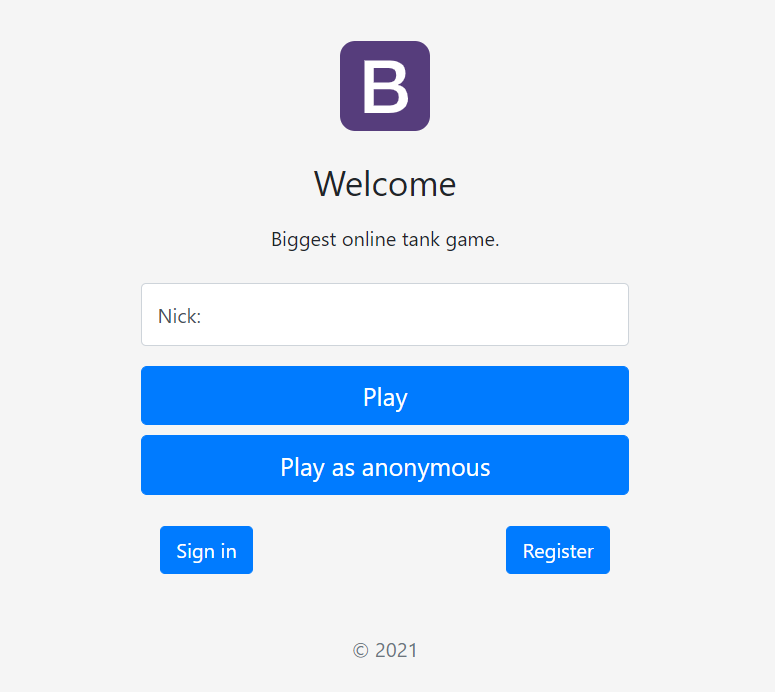
\includegraphics[width=7cm,height=7cm]{startMenu}
	\caption{Početni izbornik}
	\label{fig:opis}
\end{figure}

Prilikom registracije korisnik mora upisati e-mail adresu i lozinku koju će onda koristiti svaki sljedeći put prilikom prijave. 
Prije pokretanja same igre korisnik upisuje nadimak koji će se koristiti za prikaz rezultata trenutno aktivne runde u gornjem desnom kutu ekrana. Nakon pokretanja korisnik je automatski pozicioniran na mapu s ostalim igračima te igra započinje. Na mapama se nalaze razne prepreke i zakloni gdje se igrač može skloniti od protivnika. Također, igrica automatski spaja igrače slične jačine (broja bodova) u iste igre tako da igra bude što zanimljivija i ravnopravnija.

Registriranim korisnicima se prati broj rundi u kojima su sudjelovali te prikazuje statistika pobjeda u izborniku „Moj račun“. Nadalje, registrirani korisnici imaju mogućnost promjene izgleda njihovog oklopnog vozila u tom istom izborniku, klikom na željeni izgled među dostupnima. Izgledi se otključavaju ovisno o postignutim bodovima igrača. Korisnički izbornik nudi i mogućnost promjene zaporke, resetiranja statistike, brisanja računa i pregled statistike drugih registriranih korisnika pretraživanje po nadimku.
Unutar same web aplikacije postoji uloga administratora. Administrator ima posebno sučelje unutar kojeg ima niz opcija. Jedna od opcija je određivanje liste mapa koje su trenutno aktivne unutar same igre od ponuđenih. Daljnje opcije su pretraga korisnika po nadimku, prikaz statistike, zabranjivanje korisnicima pristup igri te uklanjanje korisnika.
Trenutno aktivna runda u donjem desnom kutu ima prozor za razgovor. Koristeći taj prozor igrači mogu izmjenjivati poruke. 

Ideju i motivaciju za igru pronašli smo u sličnim popularnim igrama namijenjenim za više igrača. Jedan od primjera je AZ Tank Game sa slike 2.2, igra s vrlo sličnom tematikom međutim namijenjena samo za igru 1 na 1. \\

\begin{figure}[h]
	\centering
	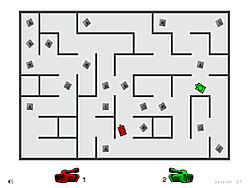
\includegraphics[width=7cm,height=7cm]{AZtankGame}
	\caption{AZ Tank Game}
	\label{fig:opis}
\end{figure}



\textit Također, igre poput Agar.io i Slither.io koje su tematski različite, ali idejno iste kao Tanky, čija smo rješenja i implementaciju proučavali kako bi dobili ideje za razvoj naše igrice.

Na slici 2.3 prikazana je igrica Slither.io koja je također namijenjena za više korisnika koji igraju jedan protiv drugog. Međutim za razliku od Tanky-a gdje je cilj pogoditi protivnika projektilom ovdje igrači pokušaju natjerati protivnike da se zabiju u tijelo njihove „zmije“ te ih tako eliminirati iz igre.

\begin{figure}[h]
	\centering
	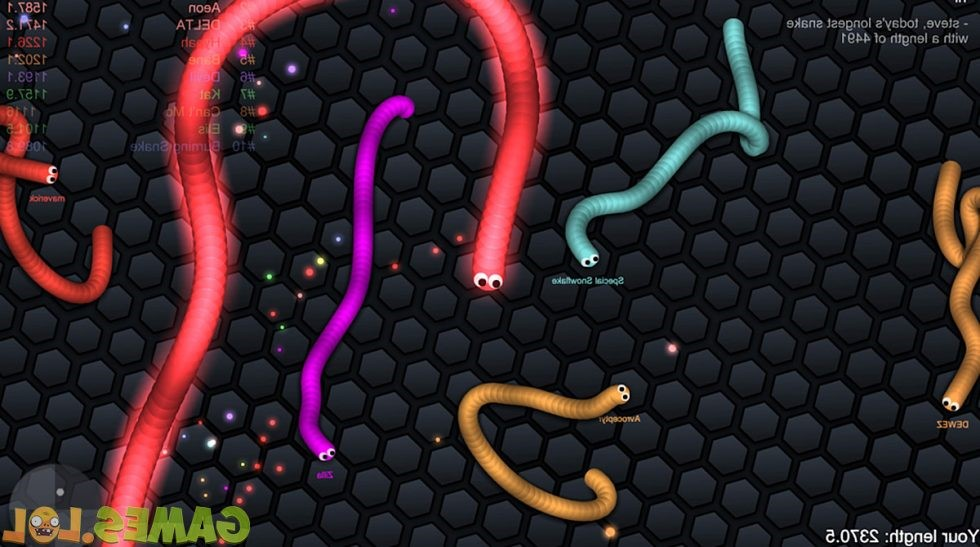
\includegraphics[width=7cm,height=7cm]{ioExample}
	\caption{Slither.io}
	\label{fig:opis}
\end{figure}

Problematizacija i opseg zadatka svodi se na razvoj back-end i front-end dijelova aplikacije u skladu s objektno orijentiranom paradigmom te na osmišljanje i izradu dizajna pojedinih elemenata. Za front-end implementaciju koristili smo HTML, CSS i JavaScript. Za back-end razvoj koristili smo Javascript, SQL te sustav za upravljanje bazama PostgreSQL u kojem smo postavili bazu podataka.

Projekt je sklon brojnim nadogradnjama koje je moguće provesti. Jedna od njih je uvođenje mogućnosti formiranja timova unutar igre. Tim bi se sastojao od minimalno dva igrača. Kreiranje runde bilo bi moguće samo za timove u kojima je isti broj igrača. Također, jedna od nadogradnji je uvođenje lige. U ligu bi mogli ući samo igrači koji su ostvarili potreban kvalifikacijski broj bodova. Liga bi se održavala 3 dana u tjednu. Kvalificirani igrač odigrao bi određen broj rundi i bio plasiran prema svom dostignuću, a isto tako i nagrađen poboljšanjima tenka.\\
 		
	
	\chapter{Specifikacija programske potpore}
		
	\section{Funkcionalni zahtjevi}			
			
			\noindent \textbf{Dionici:}
			
			\begin{packed_enum}
				
				\item Korisnik
				\begin{packed_enum}
					\item Anonimni korisnik
					\item Registrirani korisnik		
				\end{packed_enum}
				\item Administrator
				
			\end{packed_enum}
			
			\noindent \textbf{Aktori i njihovi funkcionalni zahtjevi:}
			
			
			\begin{packed_enum}
				\item  \underbar{anonimni korisnik (inicijator) može:}
				
				\begin{packed_enum}
					
					\item pridružiti se igri kao anoniman korisnik
					\begin{packed_enum}						
						\item  sustav mu dodjeljuje nadimak 				
					\end{packed_enum}
					
				\end{packed_enum}
			
				\item  \underbar{registrirani korisnik (inicijator) može:}
				
				\begin{packed_enum}
					
					\item unijeti nadimak i zaporku
					\item pratiti vlastitu statistiku u igri
					\item promijeniti izgled vozila u izborniku
					\item brisati svoj račun
					
				\end{packed_enum}
				\item  \underbar{administrator (inicijator) može:}
					\begin{packed_enum}
						\item uređivati liste mapa aktivnih unutar igre
						\item pretraživati korisnika po nadimku i vidjeti prikaz njegove statistike
						\item pretraživati najbolje igrače
					\end{packed_enum}
				
				\item  \underbar{baza podataka (sudionik) može:}
				\begin{packed_enum}
					\item pohraniti podatke o korisniku
				\end{packed_enum}

			\end{packed_enum}
			
			\eject 
			
			
				
			\subsection{Obrasci uporabe}
			
				
				\subsubsection{Opis obrazaca uporabe}
					

					\noindent \underbar{\textbf{UC1 - registracija}}
					\begin{packed_item}
	
						\item \textbf{Glavni sudionik: }Neregistriran korisnik
						\item  \textbf{Cilj:} Stvoriti korisnički račun
						\item  \textbf{Sudionici:} Baza podataka
						\item  \textbf{Preduvjet:} -
						\item  \textbf{Opis osnovnog tijeka:}
						
						\item[] \begin{packed_enum}
	
							    \item Korisnik odabire gumb za registraciju
    							\item Korisnik unosi potrebne podatke – nadimak i zaporku
    							\item Provjerava se ispravnost podataka
    							\item Podaci se spremaju u bazu podataka
   								 \item Korisnik je uspješno registriran 
						\end{packed_enum}
						
						\item  \textbf{Opis mogućih odstupanja:}
						
						\item[] \begin{packed_item}
	
							\item[2.b] Korisnik unosi već korištene podatke
							\item[] \begin{packed_enum}
								
								\item Korisnik prima obavijest da se podaci koriste
								\item Omogućava se ponovni pokušaj korisniku
								
							\end{packed_enum}
							
						\end{packed_item}
					\end{packed_item}

										\noindent \underbar{\textbf{UC2 - prijava u sustav}}
					\begin{packed_item}
	
						   \item \textbf{Glavni sudionik: } Registriran korisnik
						   \item  \textbf{Cilj:} Korištenje mogućnosti registriranog korisnika
						   \item  \textbf{Sudionici:} Baza podataka
				 	   	   \item  \textbf{Preduvjet:} Korisnik je registriran
							\item  \textbf{Opis osnovnog tijeka:}
	
					\item[] \begin{packed_enum}
		
							\item Korisnik odabira gumb "Prijava"
							\item Korisnik upisuje korisničko ime i zaporku
							\item Provjerava se ispravnost podataka
							\item Korisnik je uspješno prijavljen
				\end{packed_enum}
	
					\item  \textbf{Opis mogućih odstupanja:}
	
						\item[] \begin{packed_item}
		
						\item[2.b] 
						\item[] \begin{packed_enum}
			
									\item Korisnik nije registriran
								\item Korisnik je unio krive podatke 
			
								\end{packed_enum}
		
						\end{packed_item}
				\end{packed_item}		
					
										\noindent \underbar{\textbf{UC3 - pregled vlastite statistike}}
					\begin{packed_item}
	
						\item \textbf{Glavni sudionik: }Registrirani korisnik
						\item  \textbf{Cilj:} Praćenje broja odigranih rundi i statistika pobjeda
						\item  \textbf{Sudionici:} Baza podataka
						\item  \textbf{Preduvjet:} Korisnik je registriran(UC1)
						\item  \textbf{Opis osnovnog tijeka:}
						
						\item[] \begin{packed_enum}
	
							    \item Korisnik odabire gumb „Moj račun“
							    \item Korisnik odabire gumb "Prikaži moju statistiku"
    							\item Korisniku piše broj odigranih rundi i pobjeda
						\end{packed_enum}
					\end{packed_item}
				
										\noindent \underbar{\textbf{UC4 - pregled statistike drugih igrača}}
					\begin{packed_item}
						
						\item \textbf{Glavni sudionik: } Registrirani korisnik
						\item  \textbf{Cilj:} Mogućnost pregleda statistike drugih registriranih korisnika pretraživanjem po nadimku
						\item  \textbf{Sudionici:} Baza podataka
						\item  \textbf{Preduvjet:} Korisnik je registriran(UC1)
						\item  \textbf{Opis osnovnog tijeka:}
						
						\item[] \begin{packed_enum}
							
							\item Korisnik odabire gumb „Moj račun“
							\item Korisnik bira polje „Pretraži igrače“
							\item U odabrano polje korisnik upisuje nadimak željenog igrača
							\item Sustav izbacuje statistiku traženog igrača iz baze podataka							
						\end{packed_enum}
						
						\item  \textbf{Opis mogućih odstupanja:}
						
						\item[] \begin{packed_item}
							
							\item[5.d] Traženi korisnik je obrisao profil					
						\end{packed_item}
					\end{packed_item}
				
										\noindent \underbar{\textbf{UC5 - resetiranje statistike}}
					\begin{packed_item}
						
						\item \textbf{Glavni sudionik: } Registrirani korisnik
						\item  \textbf{Cilj:} Mogućnost resetiranje dosadašnje statistike
						\item  \textbf{Sudionici:} Baza podataka
						\item  \textbf{Preduvjet:} Korisnik je registriran(UC1)
						\item  \textbf{Opis osnovnog tijeka:}
						
						\item[] \begin{packed_enum}
							
							\item Korisnik odabire gumb „Moj Račun“
							\item Korisnik  odabire opciju "Resetiraj statistiku"
							\item Sustav nudi korisniku u skočnom prozoru mogućnost da odustane klikom na gumb "Odustani" ili da resetira statistiku klikom na gumb "Resetiraj" 
							\item Korisnikova statistika se u bazi podatak postavi na 0
						\end{packed_enum}
					\end{packed_item}
				
				
				    	\noindent \underbar{\textbf{UC6 - odjava}}
				    \begin{packed_item}
				    	
				    	\item \textbf{Glavni sudionik: } Registrirani korisnik
				    	\item  \textbf{Cilj:} Odjaviti se iz sustava
				    	\item  \textbf{Sudionici:} -
				    	\item  \textbf{Preduvjet:} Korisnik je prijavljen u sustav (UC3)
				    	\item  \textbf{Opis osnovnog tijeka:}
				    	
				    	\item[] \begin{packed_enum}
				    		
				    		\item Korisnik zahtjeva odjavu iz sustava odabirom gumba "Odjava" na početnoj stranici
				    		\item Sustav odjavljuje korisnika
				    		\item Prikazuje se početna stranica
				    	\end{packed_enum}
				    \end{packed_item}
						
					
										\noindent \underbar{\textbf{UC7 - promjena osobnih podataka}}
					\begin{packed_item}
	
						\item \textbf{Glavni sudionik: } Registrirani korisnik
						\item  \textbf{Cilj:} Mogućnost promijene zaporke
						\item  \textbf{Sudionici:} Baza podataka
						\item  \textbf{Preduvjet:} Korisnik je registriran
						\item  \textbf{Opis osnovnog tijeka:}
						
						\item[] \begin{packed_enum}
	
							    \item Korisnik odabire gumb „Moj račun“
    							\item Korisnik odabire opcije za promjenu zaporke
    							\item Korisnik upisuje novu zaporku
    							\item Korisnik sprema promjene
    							\item Baza podataka se ažurira
						\end{packed_enum}
						
						\item  \textbf{Opis mogućih odstupanja:}
						
						\item[] \begin{packed_item}
	
							\item[5.d] Korisnik je upisao novu zaporku, ali nije spremio promjene
							\item[] \begin{packed_enum}
								
								\item  Sustav obavještava korisnika da nije spremio prije izlaska iz izbornika
								
							\end{packed_enum}
							
						\end{packed_item}
					\end{packed_item}
					
										\noindent \underbar{\textbf{UC8 - promjena izgleda vozila}}
					\begin{packed_item}
	
						\item \textbf{Glavni sudionik: } Registrirani korisnik
						\item  \textbf{Cilj:} Mogućnost promjene izgleda vozila među dostupnima
						\item  \textbf{Sudionici:} Baza podataka
						\item  \textbf{Preduvjet:} Korisnik je registriran
						\item  \textbf{Opis osnovnog tijeka:}
						
						\item[] \begin{packed_enum}
	
							    \item Korisnik odabire gumb „Moj Račun“
    							\item Korisnik  odabire opciju "Odaberi novi izgled"
    							\item Korisniku se prikazuje lista otključanih izgleda koje mu dodjeljuje sustav ovisno o broju pobjeda
						\end{packed_enum}
					\end{packed_item}
				
									\noindent \underbar{\textbf{UC9 - brisanje korisničkog računa}}
					\begin{packed_item}
						
						\item \textbf{Glavni sudionik: } Registrirani korisnik
						\item  \textbf{Cilj:} Obrisati korisnički račun
						\item  \textbf{Sudionici:} Baza podataka
						\item  \textbf{Preduvjet:} Korisnik je registriran
						\item  \textbf{Opis osnovnog tijeka:}
						
						\item[] \begin{packed_enum}
							
							\item Korisnik odabire gumb „Moj Račun“
							\item Korisnik  odabire opciju „Obriši račun“
							\item Korisnički račun se briše iz baze podataka
						\end{packed_enum}
					\end{packed_item}
					
					
								\noindent \underbar{\textbf{UC10 - odabir akcije nakon smanjena zdravlja igrača na 0}}
					\begin{packed_item}
						
						\item \textbf{Glavni sudionik: } Korisnik
						\item  \textbf{Cilj:} Korisnik može odlučiti hoće li napustiti igru ili će se vratiti nakon što mu je zdravlje smanjeno na 0
						\item  \textbf{Sudionici:} -
						\item  \textbf{Preduvjet:} -
						\item  \textbf{Opis osnovnog tijeka:}
						
						\item[] \begin{packed_enum}
							
							\item Korisniku je zdravlje smanjeno na 0 te ga se izbacuje iz trenutno aktivne runde
							\item Korisniku se pojavljuje skočni prozor 
							\item Korisnik odabire jednu od ponuđenih opcija
							\item Ako odabere "Napusti" on izlazi iz aktivne igre
							\item Ako odabere "Povratak u igru" on se vraća u aktivnu rundu
						\end{packed_enum}
						
						\item  \textbf{Opis mogućih odstupanja:}
						
						\item[] \begin{packed_item}
							
							\item[5.b] 
							\item[] \begin{packed_enum}
								
								\item Ako je u trenutku povratka u igru igra završila, sustav odbija vratit korisnika u igru
								\item Ako se korisnik želi vratiti u igru, mora pričekati 30 sekundi od izbacivanja 
								
							\end{packed_enum}
							
						\end{packed_item}
					\end{packed_item}
				
				    				\noindent \underbar{\textbf{UC11 - komuniciranje između igrača}}
				    \begin{packed_item}
				    	
				    	\item \textbf{Glavni sudionik: } Korisnici(Registrirani, anonimni)
				    	\item  \textbf{Cilj:} Mogućnost komunikacije između igrača unutar runde
				    	\item  \textbf{Sudionici:} Korisnici
				    	\item  \textbf{Preduvjet:} -
				    	\item  \textbf{Opis osnovnog tijeka:} 
				    	
				    	\item[] \begin{packed_enum}
				    		
				    		\item Korisnik klikom miša odabire tekstno polje na ekranu
				    		\item Korisnik piše poruku i šalje ostalim igračima
				    	\end{packed_enum}
				    \end{packed_item}
			    
			    					\noindent \underbar{\textbf{UC12 - ulazak korisnika u rundu}}
			    	\begin{packed_item}
			    		
			    		\item \textbf{Glavni sudionik: } Korisnik (Registrirani, anonimni)
			    		\item  \textbf{Cilj:} Ulazak korisnika u rundu
			    		\item  \textbf{Sudionici:} Baza podataka
			    		\item  \textbf{Preduvjet:} -
			    		\item  \textbf{Opis osnovnog tijeka:}
			    		
			    		\item[] \begin{packed_enum}
			    			
			    			\item Korisnik odabire gumb "Igraj"
			    			\item Server korisniku dodjeljuje rundu u koju može ući
			    			\item Korisnik ulazi u rundu i igra
			    		\end{packed_enum}
			    	
		               \item  \textbf{Opis mogućih odstupanja:}
		    			
		    			\item[] \begin{packed_item}
		    				
		    				\item[2.b] 
		    				\item[] \begin{packed_enum}
		    					
		    					\item Korisnik mora čekati da mu server dodjeli rundu za igru jer server raspodjeljuje s obzirom na dosadašnji uspjeh korisnika 
		    					
		    				\end{packed_enum}
		    				
		    			\end{packed_item}
	    			\end{packed_item}
			    
			    
			   						\noindent \underbar{\textbf{UC13 - prijava administratora u sustav}}
			   		\begin{packed_item}
			   			
			   			\item \textbf{Glavni sudionik: } Administrator
			   			\item  \textbf{Cilj:} Korištenje administracijskih ovlasti
			   			\item  \textbf{Sudionici:} Baza podataka
			   			\item  \textbf{Preduvjet:} Postojanje administratora 
			   			\item  \textbf{Opis osnovnog tijeka:}
			   			
			   			\item[] \begin{packed_enum}
			   				
			   				\item Administrator odabira gumb "Prijava administratora"
			   				\item Administrator upisuje ime i zaporku
			   				\item Provjerava se ispravnost podataka
			   				\item Administrator je uspješno prijavljen
			   			\end{packed_enum}
			   			
			   			\item  \textbf{Opis mogućih odstupanja:}
			   			
			   			\item[] \begin{packed_item}
			   				
			   				\item[2.b] 
			   				\item[] \begin{packed_enum}
			   					
			   					\item Ne postoji administrator s upisanim imenom
			   					\item Postoji ime administratora, ali je pogrešna zaporka
			   					
			   				\end{packed_enum}
			   				
			   			\end{packed_item}
			   		\end{packed_item}	
						
					
										\noindent \underbar{\textbf{UC14 - zabranjivanje pristupa korisniku}}
					\begin{packed_item}
	
						\item \textbf{Glavni sudionik: } Administrator
						\item  \textbf{Cilj:} Zabraniti korisnicima pristup igri
						\item  \textbf{Sudionici:} -
						\item  \textbf{Preduvjet:} -
						\item  \textbf{Opis osnovnog tijeka:}
						
						\item[] \begin{packed_enum}
	
							    \item Administrator pronalazi korisnika kojem želi zabraniti pristup
    							\item Administrator bira opciju "Blokiraj korisnika"
    							\item Administrator zabrani pristup korisniku trajno ili privremeno
						\end{packed_enum}
					\end{packed_item}
					
					
										\noindent \underbar{\textbf{UC15 - dodjela administratorskih ovlasti}}
					\begin{packed_item}
	
						\item \textbf{Glavni sudionik: } Administrator
						\item  \textbf{Cilj:} Dodavanje novog administratora u sustav
						\item  \textbf{Sudionici:} Baza podataka
						\item  \textbf{Preduvjet:} -
						\item  \textbf{Opis osnovnog tijeka:}
						
						\item[] \begin{packed_enum}
	
							    \item Administrator odabire gumb "Dodaj novog administratora"
    							\item Administrator u polje upisuje ime i zaporku
 								\item Administrator dodaje novog administratora
						\end{packed_enum}
						
						\item  \textbf{Opis mogućih odstupanja:}
						
						\item[] \begin{packed_item}
	
							\item[2.b] 
							\item[] \begin{packed_enum}
								
								\item U sustavu postoji administrator s istim imenom
								
							\end{packed_enum}
							
						\end{packed_item}
					\end{packed_item}
					
										\noindent \underbar{\textbf{UC16 - dodjela liste mape}}
					\begin{packed_item}
	
						\item \textbf{Glavni sudionik: } Administrator
						\item  \textbf{Cilj:} Odrediti liste mape koje će biti aktivne unutar igre
						\item  \textbf{Sudionici:} Baza podataka
						\item  \textbf{Preduvjet:} Nema igara u tijeku
						\item  \textbf{Opis osnovnog tijeka:}
						
						\item[] \begin{packed_enum}
	
							    \item Administrator bira opciju "Dodjela liste mapa"
    							\item Administrator odabere liste mape koje će biti aktivne unutar same igre
						\end{packed_enum}
						
						\item  \textbf{Opis mogućih odstupanja:}
						
						\item[] \begin{packed_item}
	
							\item[2.b] 
							\item[] \begin{packed_enum}
								
								\item  Postoje igre u tijeku te administrator ne može dodijeliti liste mapa
								\item  Igrači moraju pričekati da lista mapa bude dodijeljena
								
							\end{packed_enum}
							
						\end{packed_item}
					\end{packed_item}
					
										\noindent \underbar{\textbf{UC17 - pretraga najboljih igrača}}
					\begin{packed_item}
	
						\item \textbf{Glavni sudionik: } Administrator
						\item  \textbf{Cilj:} Pronaći igrače sa najviše ostvarenih bodova
						\item  \textbf{Sudionici:} Baza podataka
						\item  \textbf{Preduvjet:} -
						\item  \textbf{Opis osnovnog tijeka:}
						
						\item[] \begin{packed_enum}
	
							    \item Administrator odabire opcije "Pretraga igrača"
    							\item Administrator odabire zatim opciju "Pretraži po rezultatu"
    							\item Administrator u tekstno polje upisuje broj korisnika koje pretražuje
    							\item Administrator odabire korisnika i ima uvid u dosadašnji uspjeh
						\end{packed_enum}
					\end{packed_item}
				
										\noindent \underbar{\textbf{UC18 - brisanje korisnika}}
					\begin{packed_item}
						
						\item \textbf{Glavni sudionik: } Administrator
						\item  \textbf{Cilj:} Obrisati korisnika
						\item  \textbf{Sudionici:} Baza podataka
						\item  \textbf{Preduvjet:} Korisnik je registriran
						\item  \textbf{Opis osnovnog tijeka:}
						
						\item[] \begin{packed_enum}
							
							\item Administrator odabire opcije "Uklanjanje korisnika"
							\item Administrator u tekstno polje upisuje ime korisnika
							\item Administrator pronalazi korisnika, uklanja ga i njegove podatke iz baze podataka
						\end{packed_enum}
					\end{packed_item}	
				
			    \newpage
				\subsubsection{Dijagrami obrazaca uporabe}
				
				\begin{figure}[h]
					\centering
					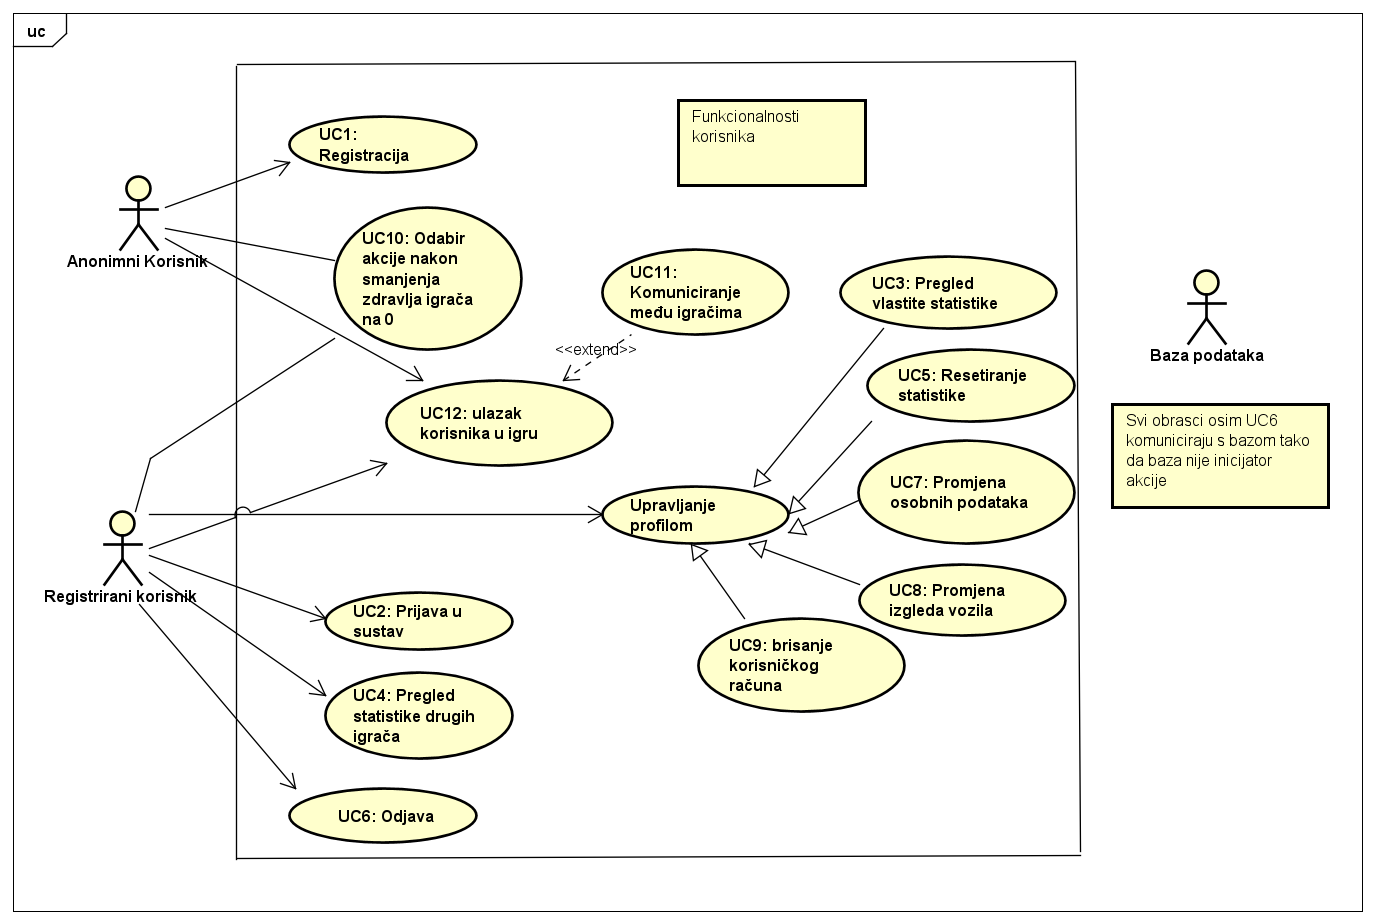
\includegraphics[width=18.5cm,height=14.5cm]{useCaseDiagram1}
					\caption{Dijagram obrazaca uporabe, funkcionalnosti korisnika}
					\label{fig:uc1}
				\end{figure}
			
			    \begin{figure}[h]
			    	\centering
			    	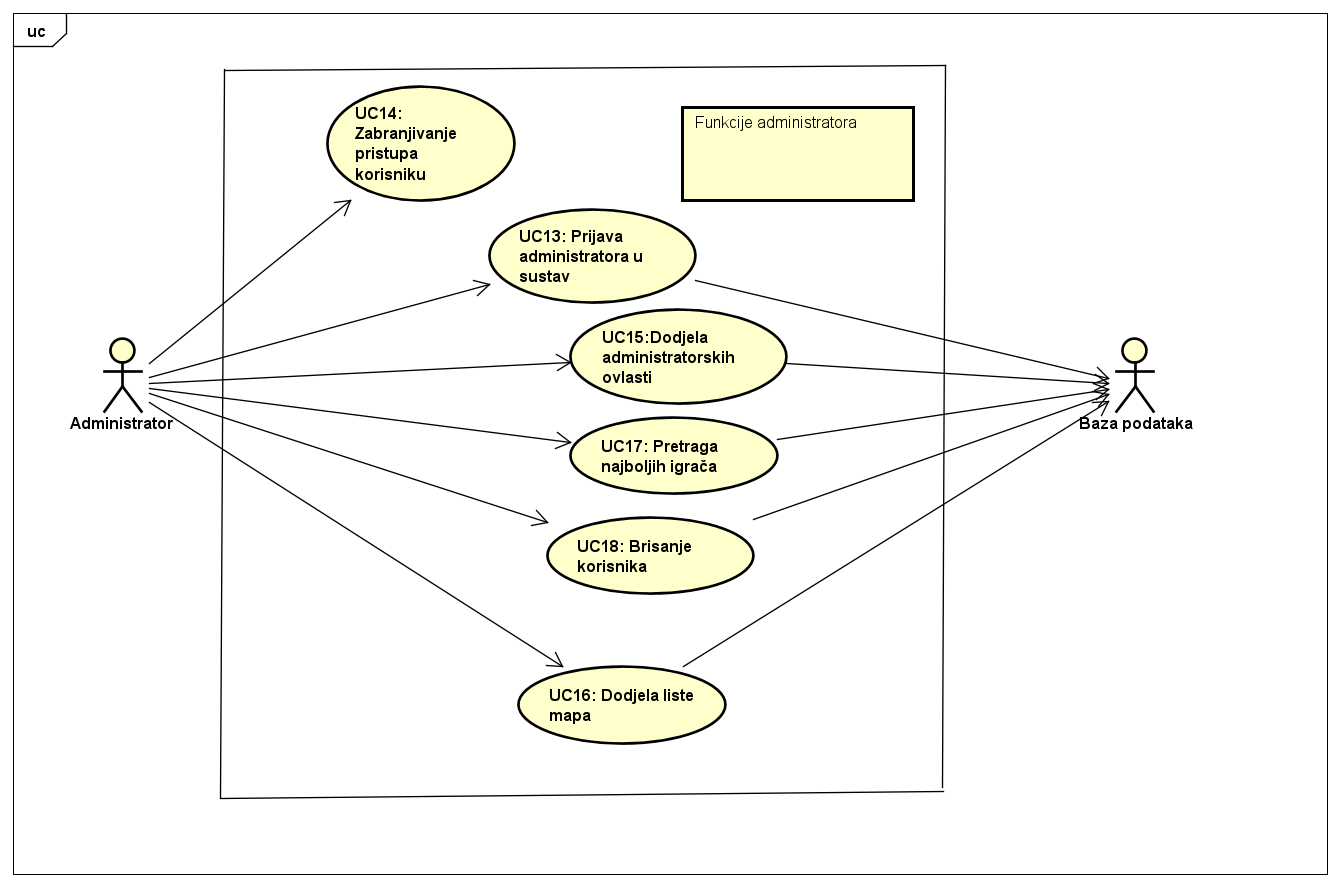
\includegraphics[width=18.5cm,height=14.5cm]{useCaseDiagram2}
			    	\caption{Dijagram obrazaca uporabe, funkcionalnosti administratora}
			    	\label{fig:uc2}
			    \end{figure}
					
				\eject		
				
				
				\newpage
			\subsection{Sekvencijski dijagrami}

			
				\textbf{\textit{Obrazac uporabe UC12 - ulazak korisnika u rundu}}\\
				\textit Korisnik želi ući u igru te odabire gumb igraj na web pregledniku. Zahtjev se šalje prema serveru. Korisnik ako je registriran ima svoju dosadašnju statistiku u bazi podataka te se prema njoj traži runda u kojoj su igrači slične razine iskustva. Ukoliko se igrača ne može svrstati u rundu u trenutku zahtjev će se slati opet dok server ne pronađe rundu u koju može korisnik ući.
				Ako u igru pak želi ući anonimni korisnik, on ima fiksan relativni učinak dodijeljen od implementiranog ELO algoritma te će se njega rasporediti u rundu s ostalim anonimnim korisnicima.\\
				
				\begin{figure}[h]
					\centering
					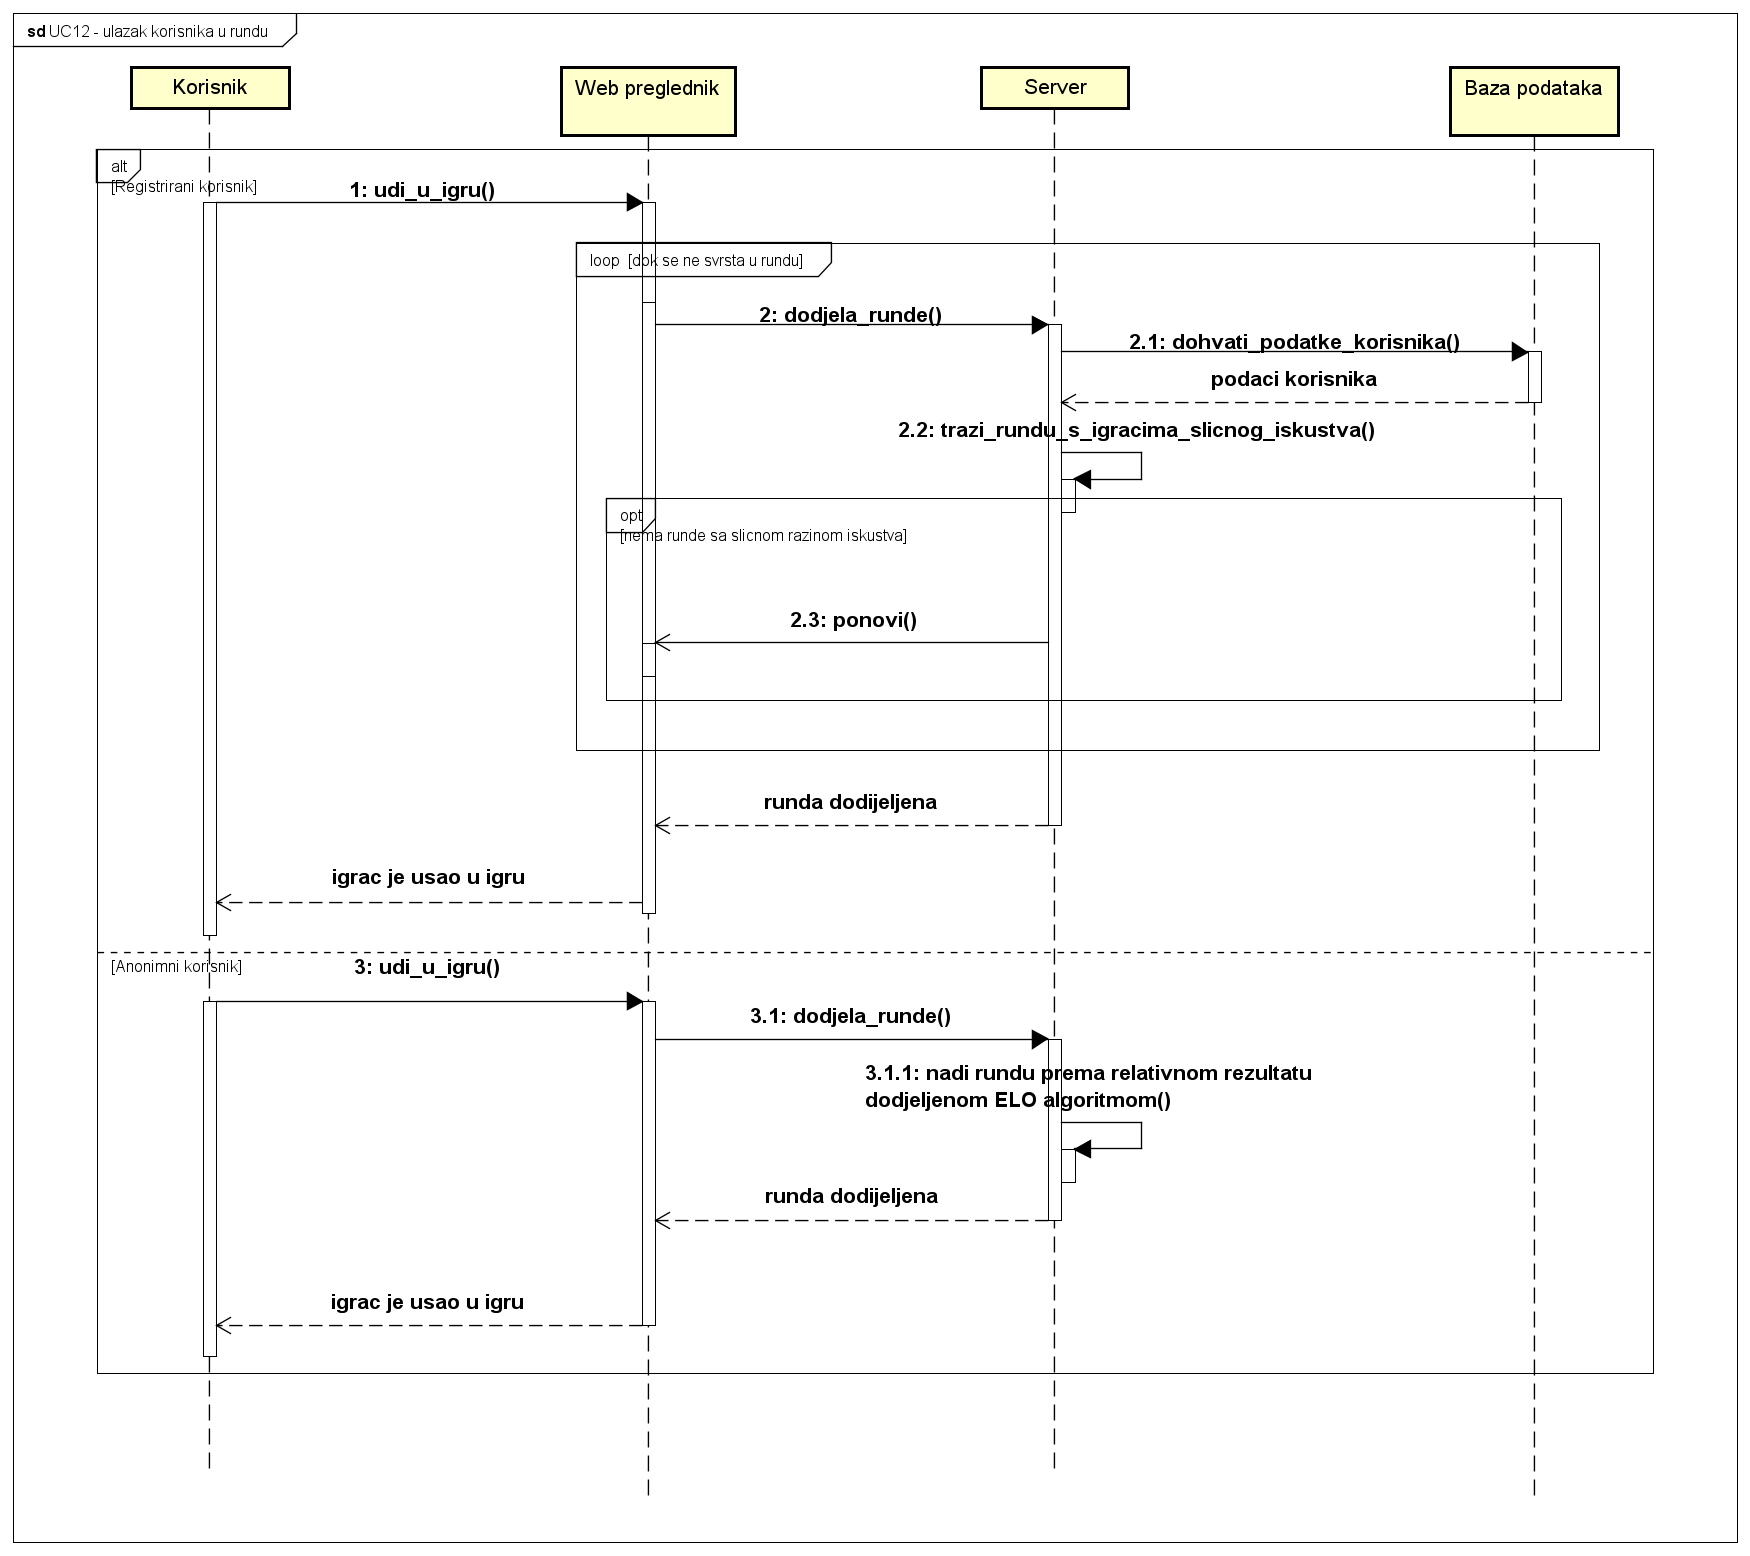
\includegraphics[width=18.5cm,height=15cm]{sequenceDiagram}
					\caption{Sekvencijski dijagram za UC12}
					\label{fig:uc12}
				\end{figure}
				
				\newpage
				\textbf{\textit{Obrazac uporabe UC3 - pregled vlastite statistike}}\\
				\textit Korisniku se pritiskom na gumb "Moj račun", kojeg vidi na web pregledniku, otvara izbornik gdje ima mogućnost odabrati gumb "Prikaži moju statistiku". Web preglednik će zahtjev za tom akcijom poslati serveru koji taj zahtjev šalje direktno bazi podataka. Baza podataka zatim pronađe statistiku traženog igrača i vraća podatke serveru. Server zatim šalje podatke web pregledniku, a na samom web pregledniku korisnik zatim može vidjeti svoju najnoviju statistiku.\\
				
				\begin{figure}[h]
					\centering
					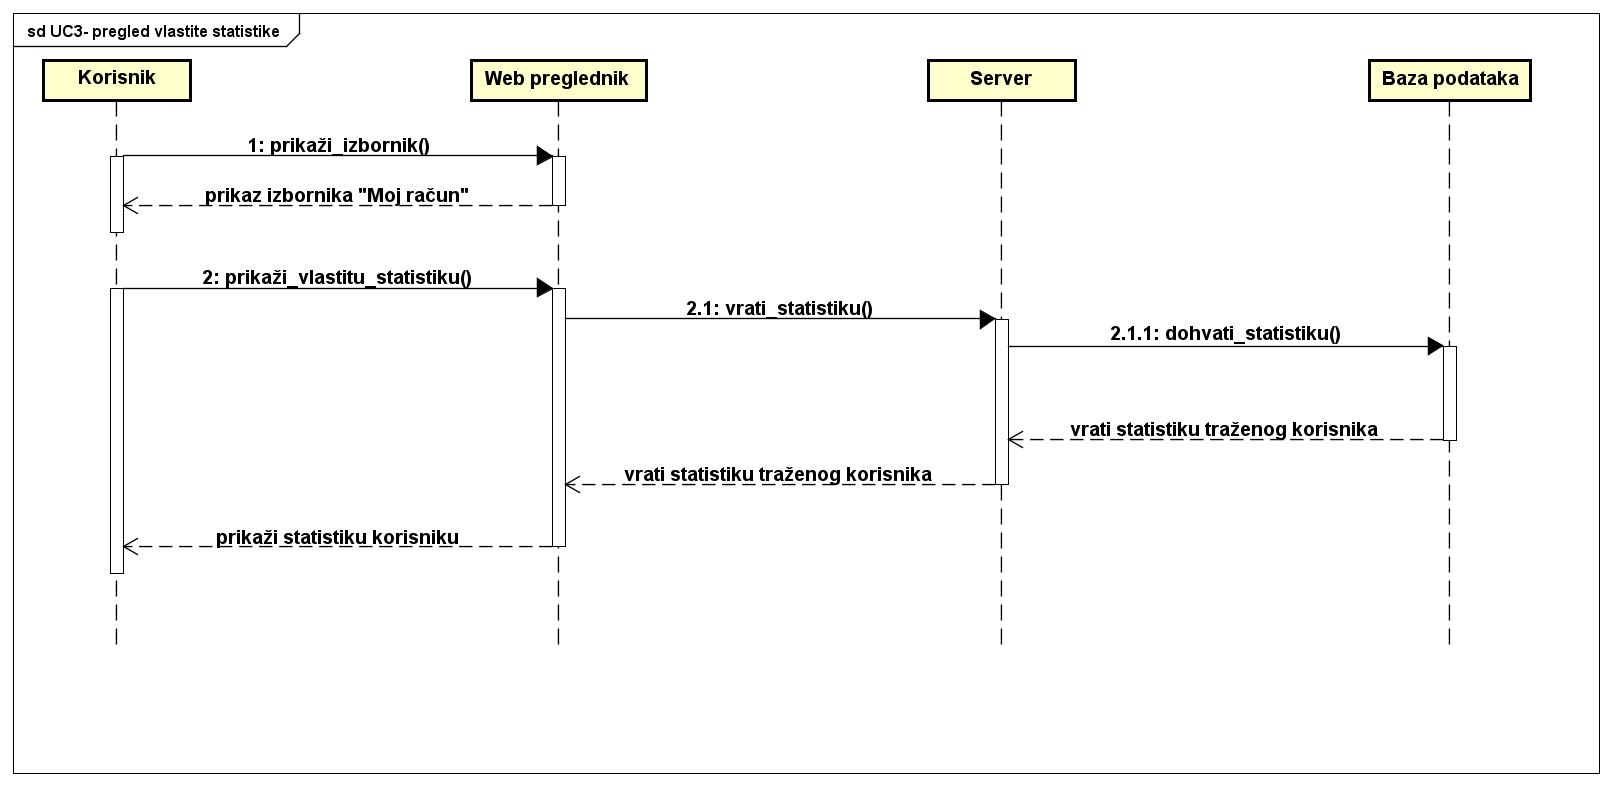
\includegraphics[width=17cm,height=12cm]{sequenceDiagram2}
					\caption{Sekvencijski dijagram za UC3}
					\label{fig:uc3}
				\end{figure}
				

				\newpage
		\section{Ostali zahtjevi}

			 \begin{enumerate}
			 	\item Prilikom registracije sustav mora upozoriti korisnika da je korisničko ime već zauzeto.
			 	\item Sustav mora podržati istodobno barem jednog administratora i barem 4 redovna korisnika.
			 	\item Sustav mora biti jednostavan za korištenje, a sučelje mora biti jasno i intuitivno.
			 	\item Sustav mora podržati hrvatske dijakritičke znakove za korisnička imena i prilikom komunikacije u prozoru za poruke.
			 	\item Sustav se temelji na HTML-u, CSS-u i JavaScriptu na korisničkoj strani te Node.js-u s express-om na serverskoj strani. 
			 	\item Koristi protokol HTTPS za komunikaciju između servera i preglednika weba.
			 	\item Sustav podržava do 50 korisnika.
			 	\item Korisnički podaci moraju biti zaštićeni nekim od algoritama enkripcije.
			 	\item Traženje nove igre ne smije trajati dulje od 5 minuta.
			 	\item Sve naknadne nadogradnje sustava ne smiju narušavati prijašnje funkcionalnosti sustava.
			 	\item Igrici se može pristupiti HTTPS-om iz javne mreže.
			 \end{enumerate}
			 
			 
	
	\chapter{Arhitektura i dizajn sustava}
		
	
	Arhitektura se može podijeliti na tri podsustava:
	\begin{enumerate}
		\item Web poslužitelj
		\item Web aplikacija
		\item Baza podataka
	\end{enumerate}
	
	\underline{Web preglednik} je program koji korisniku omogućuje pregled web-stranica i multimedijalnih sadržaja vezanih uz njih. Svaki internetski preglednik je prevoditelj. Dakle, stranica je pisana u kodu koji preglednik nakon toga interpretira kao nešto svakome razumljivo. Korisnik putem web preglednika šalje zahtjev web poslužitelju.
	
	\underline{Web poslužitelj} osnova je rada web aplikacije. Njegova primarna zadaća je komunikacija klijenta s aplikacijom. Komunikacija s odvija preko HTTPS protokola (engl. \textit{Hyper Text Transfer Protocol Secure}) protokola, koji je protokol u prijenosu informacija na webu. Poslužitelj je onaj koji pokreće web aplikaciju te joj prosljeđuje zahtjev.
	
	Korisnik koristi \underline{web aplikaciju} za obrađivanje željenih zahtjeva. Web aplikacija obrađuje zahtjev te ovisno o zahtjevu pristupa bazi podataka nakon čega preko poslužitelja vraća korisniku odgovor u obliku HTML dokumenta vidljivog u web pregledniku. Programski jezik kojeg smo odabrali za izradu naše web aplikacije je JavaScript te Express radni okvir. Odabrana razvojna okolina je Visual Studio Code. Express podržava MVC koncept i time olakšava razvoj web aplikacije. Arhitektura same aplikacije je podijeljena ne klijentski i poslužiteljski dio. Klijentski dio je izgrađen pomoću HTML-a i JavaScripta. Klijentski dio korisnici koriste za interakciju s aplikacijom kroz web preglednik. Klijentski dio šalje zahtjeve poslužitelju ovisno o akcijama korisnika. Poslužiteljski dio izgrađen je pomoću Express razvojnog okvira te primjenjuje MVC koncept. Karakteristika takvog pristupa je razdvajanje domena problema koja rezultira učinkovitijom podjelom članova po timovima. MVC također doprinosi i modularnosti koda i njegovoj čitljivosti.

	
		

		

				
		\section{Baza podataka}

		
		Za potrebu našeg sustava koristiti ćemo relacijsku bazu podataka koja svojom strukturom olakšava modeliranje interakcije u sustavu. Osnovna gradivna jedinica baze je relacija, to jest imenovana tablica s definiranim atributima. Zadaća baze podataka je brza, jednostavna i robusna pohrana, alteracija i dohvat podataka za daljnju obradu. Baza podataka ove aplikacije sastoji se od sljedećih entiteta:
		
		\begin{itemize}
			\item Korisnik
			\item Ima izgled
			\item Tenk
			\item Igrao je
			\item Igra
			\item Mapa

		\end{itemize}
		
			\subsection{Opis tablica}
				
			\textbf{Korisnik} Ovaj entitet sadrži sve bitne podatke o korisniku. Sadrži atribute: korisničko ime, lozinka, email, razinu ovlasti te datum rođenja. Ovaj entitet je u vezi \textit{One-to-many} s entitetom Igrao je preko korisničkog imena te u vezi \textit{One-to-many} s entitetom Ima izgled preko korisničkog imena.
				
				\begin{longtabu} to \textwidth {|X[6, l]|X[6, l]|X[20, l]|}
					
					\hline \multicolumn{3}{|c|}{\textbf{Korisnik}}	 \\[3pt] \hline
					\endfirsthead
					
					\hline \multicolumn{3}{|c|}{\textbf{Korisnik}}	 \\[3pt] \hline
					\endhead
					
					\hline 
					\endlastfoot
					
					\cellcolor{LightGreen}korisničko ime & VARCHAR	&  	jedinstveni identifikator korisnika 	\\ \hline
					lozinka	& VARCHAR & hash lozinke  	\\ \hline 
					email & VARCHAR & e-mail adresa korisnika  \\ \hline 
					razina ovlasti & INT	& razina ovlasti korisnika\\ \hline 
					
					
				\end{longtabu}
			
			\textbf{Ima izgled} Ovaj entitet je spojni entitet entiteta Korisnik i Tenk. Sadrži atribute: korisničko ime i tenkId. Ovaj entitet je u vezi \textit{Many-to-one} s entitetom Korisnik preko korisničkog imena te u vezi \textit{Many-to-one} s entitetom Tenk preko tenkId-a.
				
				\begin{longtabu} to \textwidth {|X[6, l]|X[6, l]|X[20, l]|}
					
					\hline \multicolumn{3}{|c|}{\textbf{Ima izgled}}	 \\[3pt] \hline
					\endfirsthead
					
					\hline \multicolumn{3}{|c|}{\textbf{Ima izgled}}	 \\[3pt] \hline
					\endhead
					
					\hline 
					\endlastfoot
					
					\cellcolor{LightGreen}korisničko ime & VARCHAR	&  	jedinstveni identifikator korisnika 	\\ \hline
					\cellcolor{LightGreen}tenkId	& VARCHAR & jedinstveni identifikator tenka  	\\ \hline 
					
					
				\end{longtabu}
			
			
			\textbf{Tenk} Ovaj entitet sadržava informacije o tenku. Sadrži atribute: tenkId, ime tenka, razina otključavanja. Ovaj entitet je u vezi \textit{Many-to-many} s entitetom Ima izgled preko tenkId-a.
			
				\begin{longtabu} to \textwidth {|X[6, l]|X[6, l]|X[20, l]|}
					
					\hline \multicolumn{3}{|c|}{\textbf{Tenk}}	 \\[3pt] \hline
					\endfirsthead
					
					\hline \multicolumn{3}{|c|}{\textbf{Tenk}}	 \\[3pt] \hline
					\endhead
					
					\hline 
					\endlastfoot
					
					\cellcolor{LightGreen}tenkId & VARCHAR	&  	jedinstveni identifikator tenka 	\\ \hline
					ime tenka	& VARCHAR & naziv tenka  	\\ \hline 
					razina otključavanja & INT & razina na kojoj korisnik otključava ovaj tenk  \\ \hline 
					
					
				\end{longtabu}
			
			\textbf{Igrao je} Ovaj entitet je spojni entitet entiteta Korisnik i Igra. Sadrži atribute: korisničko ime, broj bodova, puta uništio, puta uništen te igraId. Ovaj entitet je u vezi \textit{Many-to-one} s entitetom Korisnik preko korisničkog imena te u vezi \textit{One-to-many} s entitetom Igra preko igraId.
			
				\begin{longtabu} to \textwidth {|X[6, l]|X[6, l]|X[20, l]|}
					
					\hline \multicolumn{3}{|c|}{\textbf{Igrao je}}	 \\[3pt] \hline
					\endfirsthead
					
					\hline \multicolumn{3}{|c|}{\textbf{Igrao je}}	 \\[3pt] \hline
					\endhead
					
					\hline 
					\endlastfoot
					
					\cellcolor{LightGreen}korisničko ime & VARCHAR	&  	jedinstveni identifikator korisnika 	\\ \hline
					\cellcolor{LightGreen}igraId	& INT & jedinstveni idenitifikator igre  	\\ \hline 
					puta uništio & INT & broj neprijatelja koje je korisnik uništio za vrijeme igre  \\ \hline
					puta uništen & INT & broj puta koje je korisnik bio uništen za vrijeme igre  \\ \hline
					
					
				\end{longtabu}
			
			\textbf{Igra} Ovaj entitet sadrži informacije o odigranoj igri. Sadrži atribute: igraId, vrijeme početka, vrijeme kraja, mapaId. Ovaj entitet je u vezi \textit{One-to-many} s entitetom Igrao je preko igraId-a te u vezi \textit{Many-to-one} s entitetom Mapa.
			
				\begin{longtabu} to \textwidth {|X[6, l]|X[6, l]|X[20, l]|}
					
					\hline \multicolumn{3}{|c|}{\textbf{Igra}}	 \\[3pt] \hline
					\endfirsthead
					
					\hline \multicolumn{3}{|c|}{\textbf{Igra}}	 \\[3pt] \hline
					\endhead
					
					\hline 
					\endlastfoot
					
					\cellcolor{LightGreen}igraId & SERIAL INT	&  	jedinstveni identifikator igre 	\\ \hline
					\cellcolor{LightBlue}mapaId	& INT & jedinstveni identifikator mape  	\\ \hline 
					vrijeme početka & TIMESTAMP & trenutak početka igre  \\ \hline
					vrijeme kraja & TIMESTAMP & trenutak kraja igre  \\ \hline
					
					
				\end{longtabu}
			
			\textbf{Mapa} Ovaj entitet sadrži informacije o mapama. Sadrži atribute: mapaId te zahtjevnost mape. Ovaj entitet je u vezi \textit{One-to-many} s entitetom Igra preko mapaId-a.
			
				\begin{longtabu} to \textwidth {|X[6, l]|X[6, l]|X[20, l]|}
					
					\hline \multicolumn{3}{|c|}{\textbf{Mapa}}	 \\[3pt] \hline
					\endfirsthead
					
					\hline \multicolumn{3}{|c|}{\textbf{Mapa}}	 \\[3pt] \hline
					\endhead
					
					\hline 
					\endlastfoot
					
					\cellcolor{LightBlue}mapaId	& INT & jedinstveni identifikator mape  	\\ \hline 
					zahtjevnost mape & INT & zahtjevnost mape za igrati na njoj  \\ \hline
					
					
				\end{longtabu}
				
			
			\subsection{Dijagram baze podataka}
				
				\begin{figure}[h]
					\centering
					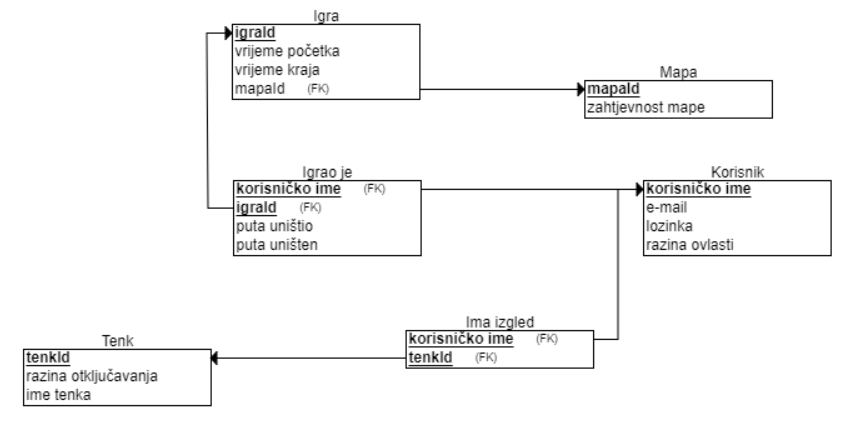
\includegraphics[width=18.5cm,height=10cm]{./databaseDiagram}
					\caption{Dijagram baze podataka}
					\label{fig:uc}
				\end{figure}
			
			\eject
			
			
		\section{Dijagram razreda}
		
		Na slici 4.2 prikazani su razredi koji pripadaju \textit{backend} dijelu MVC arhitekture. Razred Objekt je razred kojeg nasljeđuju svi objekti koji se pojavljuju na igraćem polju. Trenutno su to samo razredi Projectile i Tank. Za svaki tenk je vezana kolekcija svih projektila koje je ispalio, a da su još uvijek u igraćem polju. Također, postoji i razred Game koji reprezentira jednu igru. Budući da je moguće imati više igara u tijeku, moguće je imati i više instanci tog razreda. U jednoj igri može biti više igrača(tenkova) dok jedan igrač može trenutno biti u samo jednoj igri. U budućim iteracijama planira se više razreda objekata na mapi koji nasljeđuju razred Object. Budući da JavaScript ne razlikuje privatne, zaštićene i javne metode i atribute oni nisu ni navedeni.
			
			\begin{figure}[h]
				\centering
				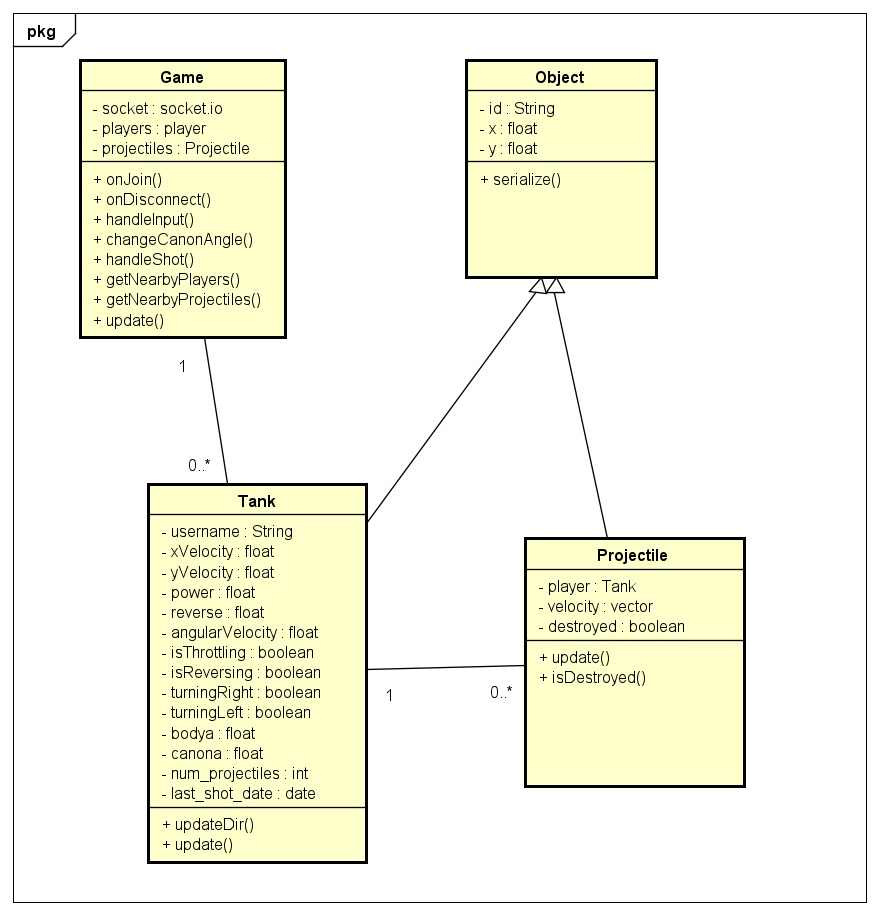
\includegraphics[width=16cm,height=12cm]{classDiagram}
				\caption{Dijagram razreda}
				\label{fig:uc}
			\end{figure}
			
			
			\newpage
			\textbf{\textit{dio 2. revizije}}\\			
			
			\textit{Prilikom druge predaje projekta dijagram razreda i opisi moraju odgovarati stvarnom stanju implementacije}
			
			
			
			\eject
		
		\section{Dijagram stanja}
			
			{UML dijagram stanja opisuje dinamičko ponašanje dijela sustava. Prikazuje stanja te prijelaze u neka druga stanja temeljene na nekim događajima. U ovom slučaju događaje određuje registrirani korisnik. Najprije, klikom na "Moj račun" korisniku se otvara izbornik s različitim mogućnostima koje može odabrati sve dok ne odluči kliknuti "Odjava". Korisnik može pregledati vlastitu statistiku ili resetirati statistiku. Kada će potvrditi resetiranje statistike, ona će se u bazi podataka postaviti na 0. Također, korisnik može pretražiti igrače. Kada odabere opciju "Pretraži igrače", automatski se pojavi polje za upis imena željenog igrača. U izborniku se nudi i promjena izgleda vozila koje je korisnik otključao. Klikom na "Promjeni podatke", korisnik može promijeniti svoje podatke tako da upiše novu zaporku i zatim spremi podatke. Korisnik može i obrisati svoj račun klikom na gumb "Obrši račun" čime će se iz baze podataka automatski korisnik obrisati. Nakon mogućih opcija koje korisnik može odabrati na "Moj račun", on također ulazi u samo igru klikom na gumb "Igraj". Nakon toga, server će tražiti rundu, ali odmah po ulasku u stanje traženja runde iz baze podataka će dobaviti podatke o iskustvu kako bi pronašao odgovarajuću rundu. Ako runda nije pronađena, postupak će se ponoviti, a u suprotnom korisnik ulazi u rundu.}
		
			
			\begin{figure}[h]
				\centering
				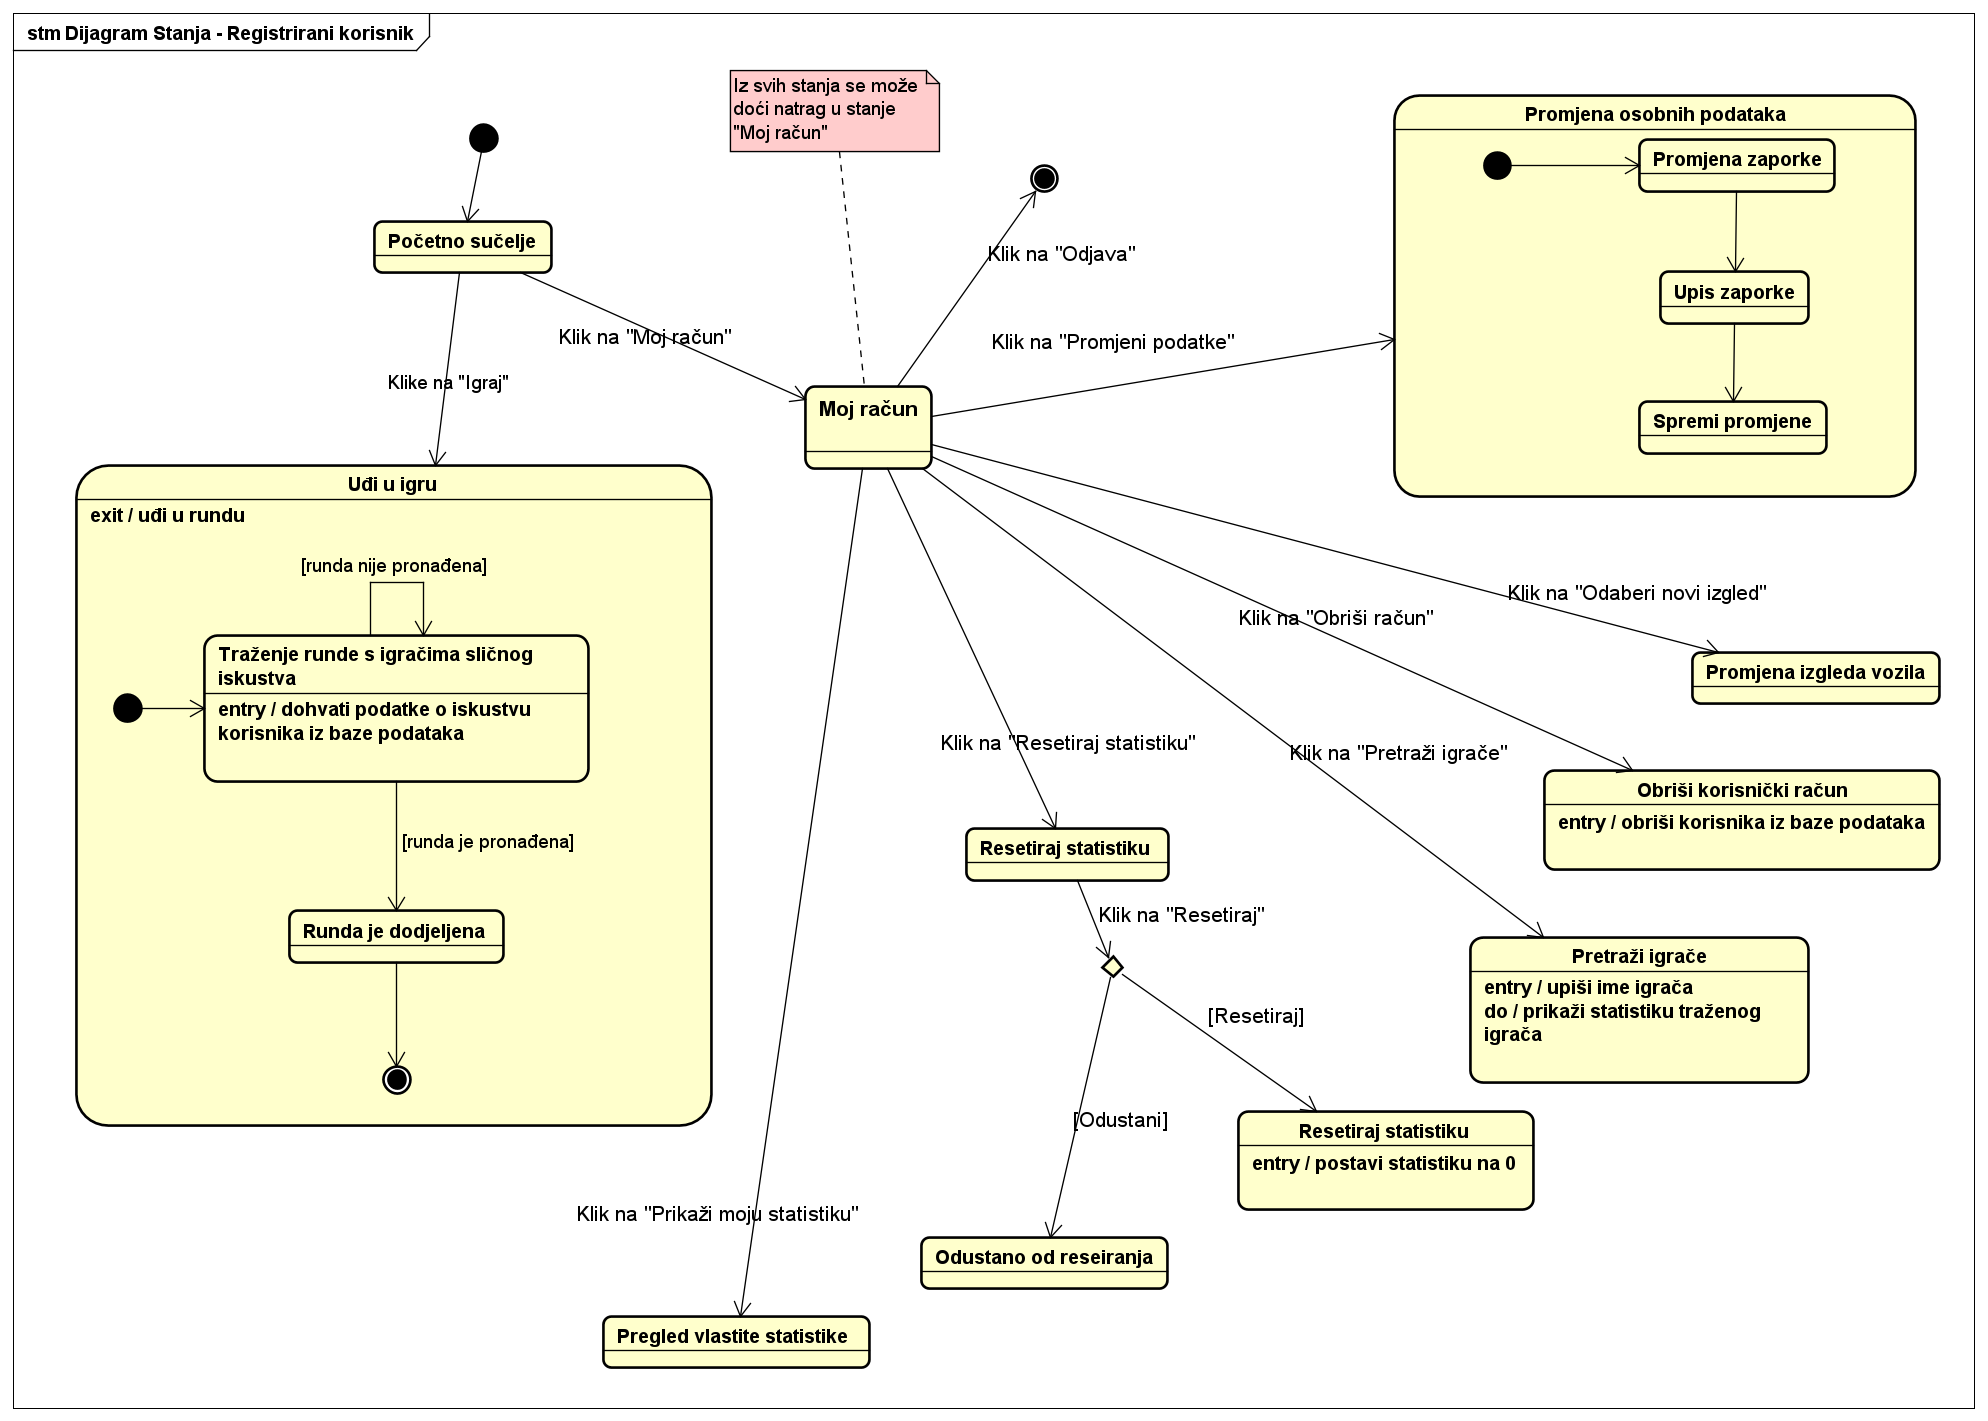
\includegraphics[width=17.5cm,height=12.5cm]{Dijagram Stanja - Registrirani korisnik}
				\caption{Dijagram stanja}
				\label{fig:stm}

			\end{figure}
			
			\eject 
			
	
		\section{Dijagram aktivnosti}
		
			{UML dijagram aktivnosti modelira ponašanja nizom aktivnosti, ali pritom se prijelaz iz jedne aktivnosti u drugu ne potiče nekim događajem. Priloženi dijagram aktivnosti prikazuje ulazak registriranog korisnika u igru. Korisnik se najprije prijavljuje u sustav sa svojim podacima. Akcije koje slijede su postupak prijave korisnika sve dok baza podataka ne vrati tražene podatke ili ih ne pronađe što znači da prijava nije uspjela. Nakon prijave, korisnik će ući u igru. Web preglednik će od servera tražiti dodjelu runde. Na serveru će se dogoditi dvije akcije. Prvo će iz baze podataka dohvatiti razinu iskustva tog korisnika, a zatim pronaći rundu s igračima slične razine iskustva. Ukoliko pronađe rundu, korisnik će uspješno ući u igru, a u suprotnom će se ponoviti traženje runde.}
			 
			\begin{figure}[h]
			 	\centering
			 	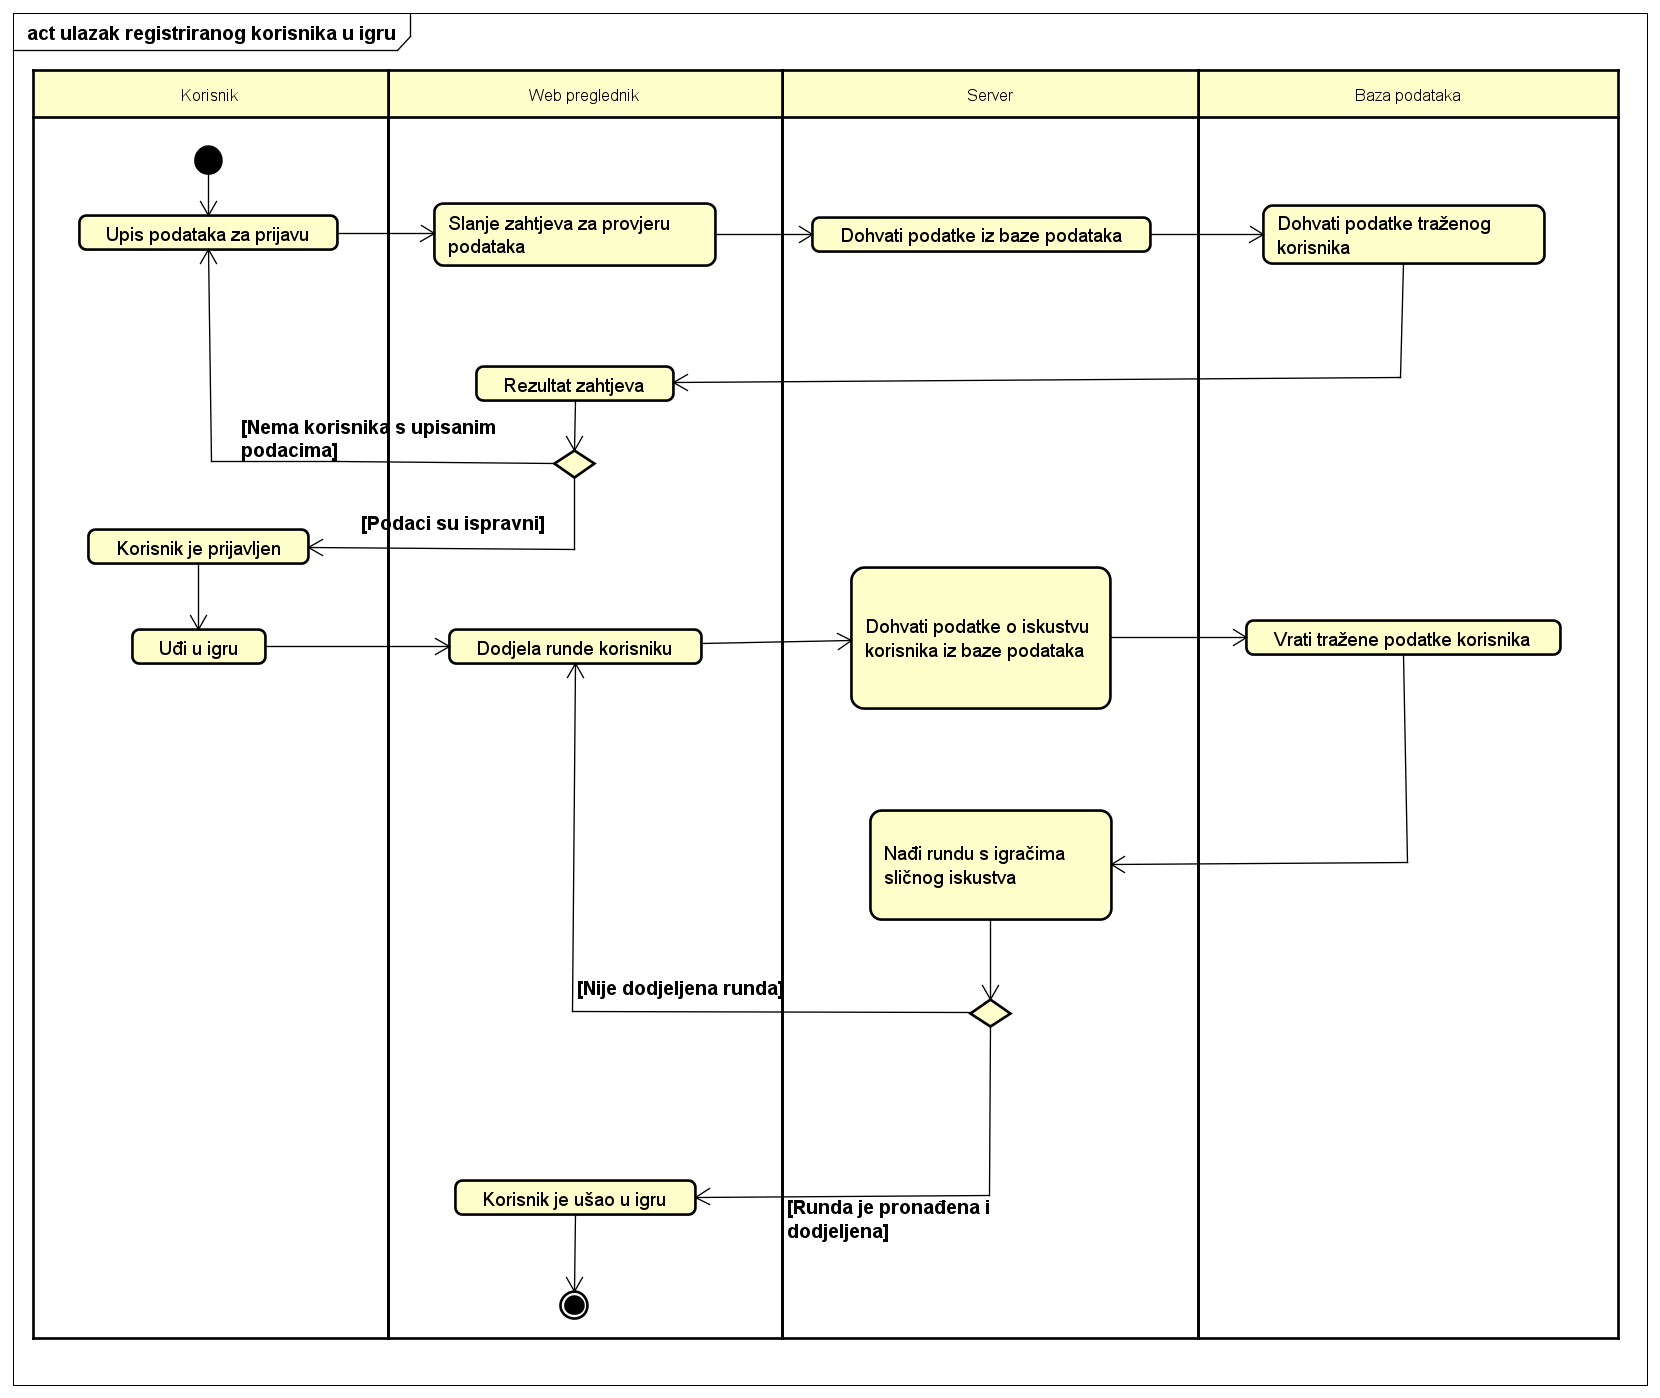
\includegraphics[width=17.5cm,height=12.5cm]{activityDiagram}
			 	\caption{Dijagram aktivnosti}
			 	\label{fig:act}
			\end{figure}
			
			\eject
		
		\newpage
		\section{Dijagram komponenti}
			
			 {Dijagram komponenti prikazuje specifikaciju arhitekture programske potpore. Vizualizira organizaciju i međuovisnosti između implementacijskih komponenata. }
			 
			 \begin{figure}[h]
			 	\centering
			 	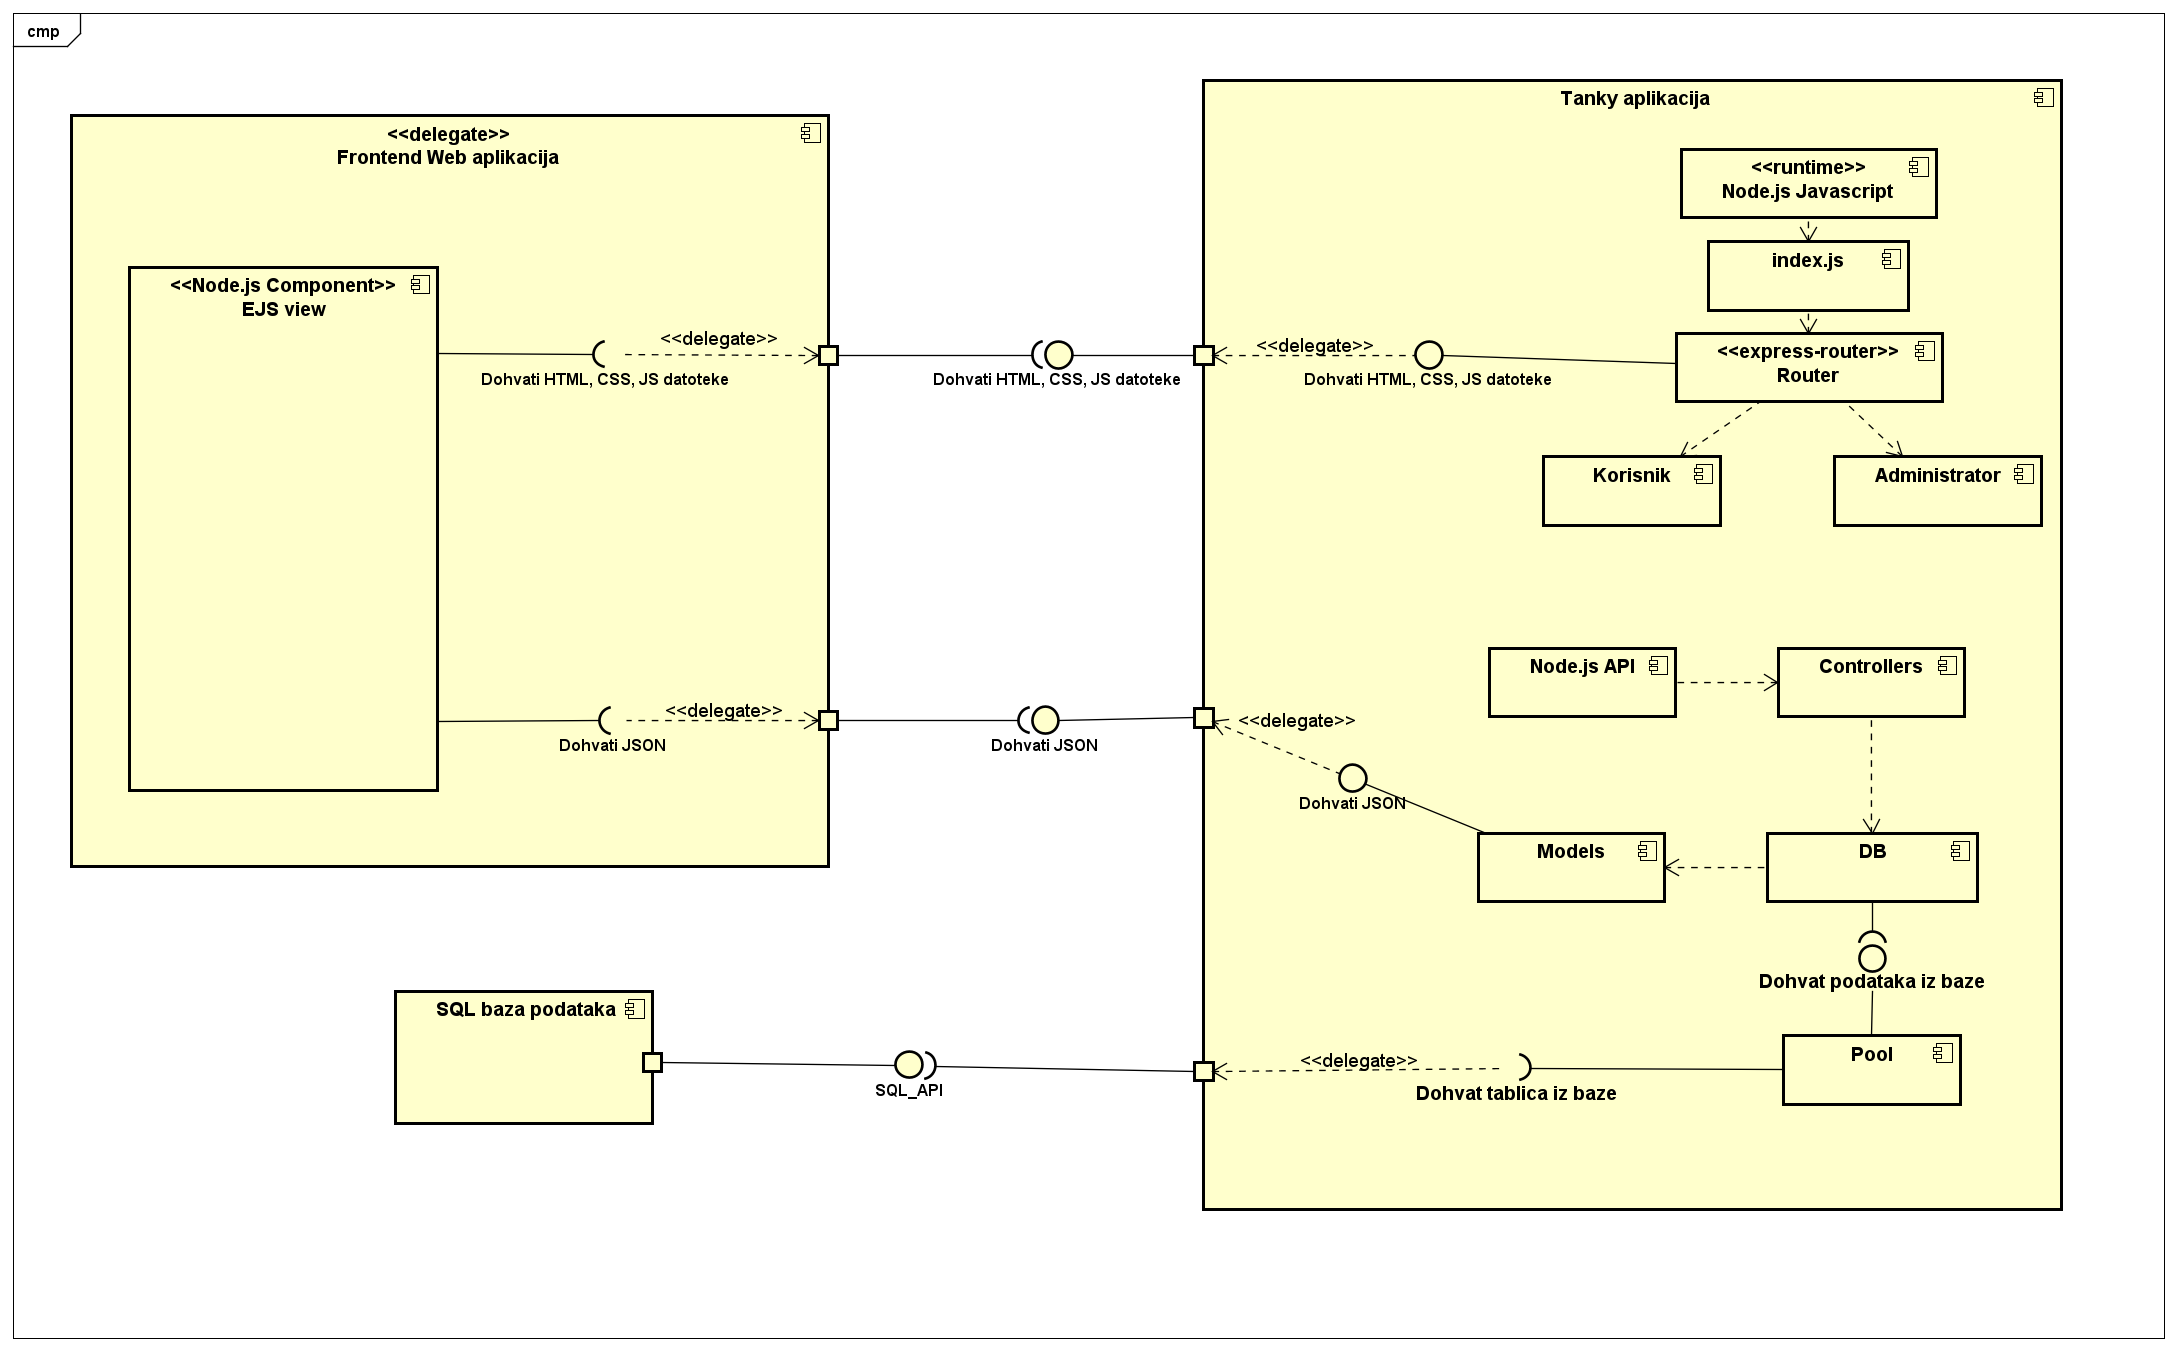
\includegraphics[width=17.5cm,height=12.5cm]{Component Diagram0}
			 	\caption{Dijagram komponenti}
			 	\label{fig:cmp}
			 \end{figure}
	\chapter{Implementacija i korisničko sučelje}
		
		
		\section{Korištene tehnologije i alati}
			
			 {Projektni tim je tijekom izrade projekta komunicirao putem Microsoft  Teams(1) i WhatsApp(2) aplikacija. Pri izradi UML dijagrama korišten je alat Astah UML(3). Kao sustav za upravljanje izbornim kodom korišten je  Git(4), a web platforma GitLab(5) koristila se kao udaljeni repozitorij.
			 Visual Studio Code(6) koristio se kao razvojna okolina za izradu projekta. Radni okvir Express(7) u kombinaciji sa serverskim okruženjem Node.js(8) korišten je za izradu aplikacije na poslužiteljskoj strani, a na klijentskoj strani korišteni su HTML(9), CSS(9) te jezik Javascript(10). Express je brz minimalistički web radni okvir za Node.js, a značajke su mu: robusno preusmjeravnje, fokus na visoke perfomanse i http pomoćne metode. Sustav za upravljanje bazom podataka korišten na ovom projektu je PostgreSQL(11). Kao pomoć pri razmještaju korišten je Digital Ocean(12).}
		 	 
		 	 \hrule
		 	 \hfill \break
		 	 {(1) https://www.microsoft.com/
		 	 \hfill \break
		 	 (2) https://web.whatsapp.com/
		 	 \hfill \break
		 	 (3) https://astah.net/products/astah-uml/
		 	 \hfill \break
		 	 (4) https://git-scm.com/
		 	 \hfill \break
		 	 (5) https://gitlab.com/
		 	 \hfill \break
		 	 (6) https://code.visualstudio.com/
		 	 \hfill \break
		 	 (7) https://expressjs.com/
		 	 \hfill \break
		 	 (8) https://nodejs.org/en/
		 	 \hfill \break
		 	 (9) https://html.com/
		 	 \hfill \break
		 	 (10) https://www.javascript.com/
		 	 \hfill \break
		 	 (11) https://www.postgresql.org/
		 	 \hfill \break
		 	 (12) https://www.digitalocean.com/
		 	 
		 	 
		 	 
		 	 
		 	 
			
			
			\eject 
		
	
		\section{Ispitivanje programskog rješenja}
			{Svi unit testovi napravljeni su nad klasom Tank koja implementira najvažnije funkcionalnosti. Napravljeni su nad fukncijama koje izazivaju moguće poteškoće u samom kodu i tokom igranja igrice. Funkcije se odnose na koliziju tanka sa objektima na mapi. Na priloženoj slici vidimo da su svi testovi uspješno prošli.}

			\subsection{Ispitivanje komponenti}
			\begin{figure}[h]
				\centering
				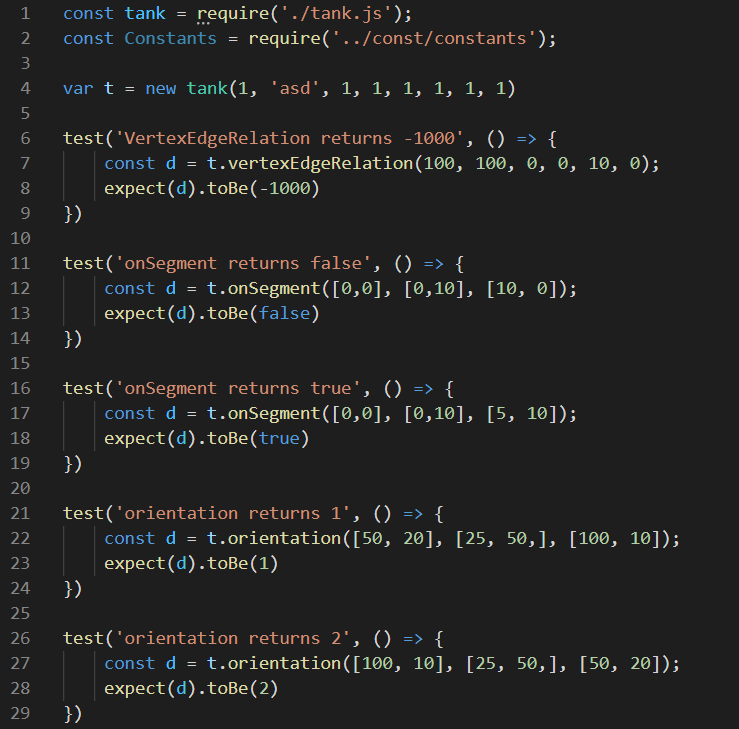
\includegraphics[width=18.5cm,height=10.5cm]{unitTests1}
				\caption{Unit testovi 1.dio}
				\label{fig:ut1}
			\end{figure}
		
			\break
			\begin{figure}[h]
				\centering
				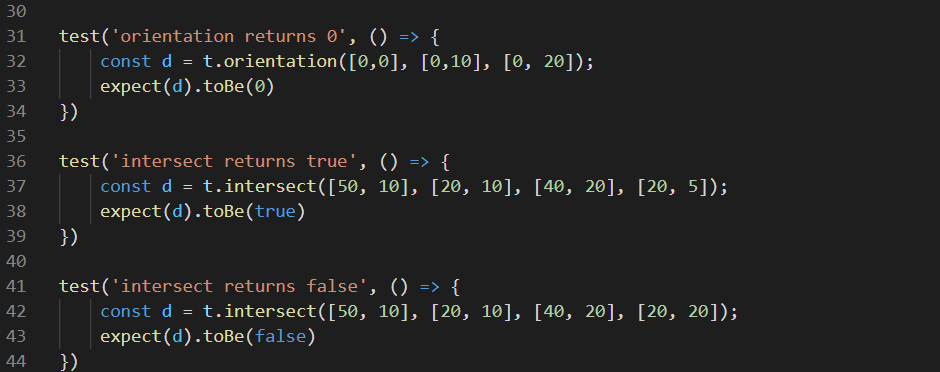
\includegraphics[width=18.5cm,height=6.5cm]{unitTest2}
				\caption{Unit testovi 2.dio}
				\label{fig:ut2}
			\end{figure}
		
		
			\begin{figure}[h]
				\centering
				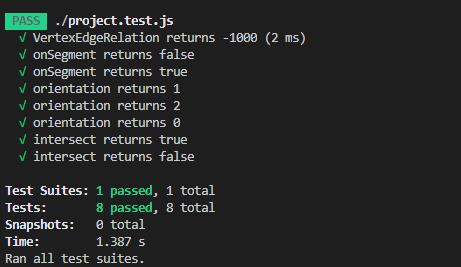
\includegraphics[width=18.5cm,height=6.5cm]{unitTestResult}
				\caption{Rezultati unit testova}
				\label{fig:ut2}
			\end{figure}
			
			
			\break
			\subsection{Ispitivanje sustava}
			
			 \textit{Potrebno je provesti i opisati ispitivanje sustava koristeći radni okvir Selenium\footnote{\url{https://www.seleniumhq.org/}}. Razraditi \textbf{minimalno 4 ispitna slučaja} u kojima će se ispitati redovni slučajevi, rubni uvjeti te poziv funkcionalnosti koja nije implementirana/izaziva pogrešku kako bi se vidjelo na koji način sustav reagira kada nešto nije u potpunosti ostvareno. Ispitni slučaj se treba sastojati od ulaza (npr. korisničko ime i lozinka), očekivanog izlaza ili rezultata, koraka ispitivanja i dobivenog izlaza ili rezultata.\\ }
			 
			 \textit{Izradu ispitnih slučajeva pomoću radnog okvira Selenium moguće je provesti pomoću jednog od sljedeća dva alata:}
			 \begin{itemize}
			 	\item \textit{dodatak za preglednik \textbf{Selenium IDE} - snimanje korisnikovih akcija radi automatskog ponavljanja ispita	}
			 	\item \textit{\textbf{Selenium WebDriver} - podrška za pisanje ispita u jezicima Java, C\#, PHP koristeći posebno programsko sučelje.}
			 \end{itemize}
		 	\textit{Detalji o korištenju alata Selenium bit će prikazani na posebnom predavanju tijekom semestra.}
			
			\eject 
		
		
		\section{Dijagram razmještaja}
		
			{Dijagram razmještaja opisuje topologiju sustava i odnos sklopovskih i programskih dijelova. Na poslužiteljskom računalu se nalaze web poslužitelj i poslužitelj baze podataka. Klijenti preko web preglednika na svom računalu pristupaju web aplikaciji. Sustav je baziran na arhitekturi ”klijent – posluzitelj”, a komunikacija između računala korisnika i poslužitelja odvija se preko HTTPS veze. Dakle, korisnik putem web preglednika šalje zahtjev web poslužitelju koji pokreće web aplikaciju i prosljeđuje joj zahtjev.}
			
			\begin{figure}[h]
				\centering
				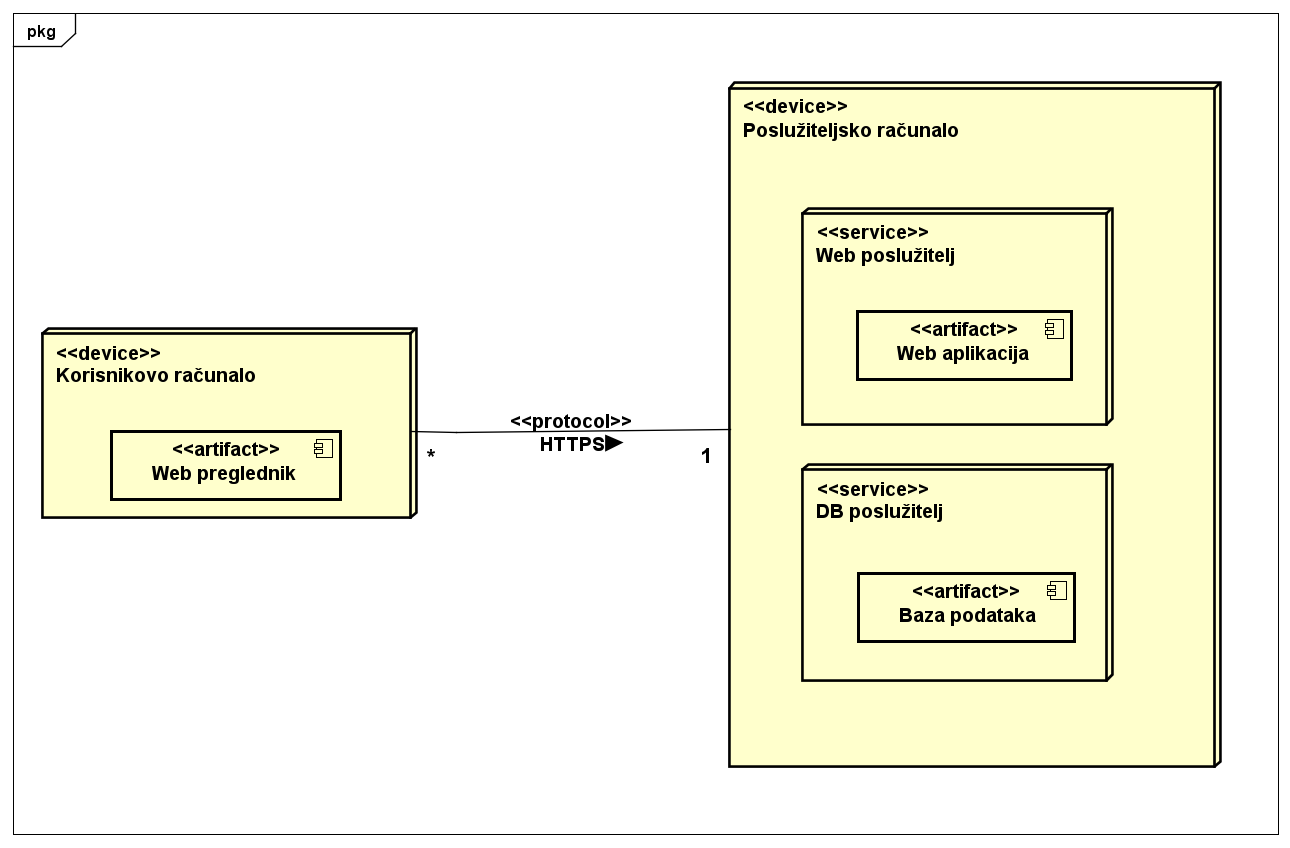
\includegraphics[width=17.5cm,height=12.5cm]{deploymentDiagram}
				\caption{Dijagram razmještaja}
				\label{fig:pkg}
			\end{figure}
			
			\eject 
		
		\section{Upute za puštanje u pogon}
		
			{Za puštanje aplikacije u pogon potreban je korisnički račun na usluzi Digital Ocean. Zapotrebe projekta, koristimo besplatnu verziju korisničkog računa. Za potrebe projekta korištena je baza podataka PostgreSQL. Konfiguracijska datoteka za bazu podataka nalazi se u datoteci izvorni\_kod/db/the\_backup.sql. Prazna baza podataka pokreće se korištenjem naredbe “psql the\_backup.sql”. Nakon toga na bazu se spaja koristeći datoteku izvorni\_kod/db/inde.js gdje se unosi korisničko ime za bazu podataka, lozinka i port. Za puštanje aplikacije u rad potrebno je klonirati repozitorij na server te pokrenuti naredbom “npm start” uz prethodno postavljanje node.js.}
			
			
			\eject 
	\chapter{Zaključak i budući rad}
		
		 {Prva faza projekta započela je okupljanjem projektnog tima i definicijom vlastitog projektnog zadatka.
		 	Tim je podijeljen na manje podtimove koji su bili specijalizirani za različita područja razvoja. Izrađeni su početni konceptualni prototipi.
		 	Prototipi su provjereni te se nastavio razvoj na najboljem. Sama igrica koja je razvijena je postavljena na Digital Ocean server te se mogla
		 	slobodno isprobati.
		 	
		 	
		 	U drugoj fazi razvoj igrice je bio u fokusu te su se dodavale nove značajke. Paralelno se igricu testiralo te su se ispravljali pronađeni problemi.
		 	Također, u drugoj fazi je dodano i korisničko sučelje za ulaz u igru, te grafika za prijavljivanje i registriranje.
		 	
		 	
		 	U trećoj fazi izgrađena je baza podataka te je izgrađena poslužiteljska strana aplikacije. U ovoj fazi je provedeno i testiranje te su dodane završne značajke za samu igru.
		 	
		 	
		 	Potencijalna nadogradnja aplikacije je dodavanje drugih modova igre te podrška za druge jezike.
		 	
		 	
		 	U radu na ovom projektu susreli smo se s raznim problemima vezanim uz neiskustvo, manjak vremena članova tima te raznovrsnosti korištenih tehnologija.
		 	Rad na ovom projektu ponudio nam je nove vještine razvoja web aplikacija te komunikacijske vještine nužno potrebne za rad u timu.}
	 	
		
		 \textit{Potrebno je točno popisati funkcionalnosti koje nisu implementirane u ostvarenoj aplikaciji.}
		
		\eject 
	\chapter*{Popis literature}
		\addcontentsline{toc}{chapter}{Popis literature}
		
		
		\begin{enumerate}
			
			\item  Programsko inženjerstvo, FER ZEMRIS, \url{http://www.fer.hr/predmet/proinz}
			
			\item  I. Sommerville, "Software engineering", 8th ed, Addison Wesley, 2007.
			
			\item  T.C.Lethbridge, R.Langaniere, "Object-Oriented Software Engineering", 2nd ed. McGraw-Hill, 2005.
			
			\item  I. Marsic, Software engineering book``, Department of Electrical and Computer Engineering, Rutgers University, \url{http://www.ece.rutgers.edu/~marsic/books/SE}
			
			\item  The Unified Modeling Language, \url{https://www.uml-diagrams.org/}
			
			\item  Astah Community, \url{http://astah.net/editions/uml-new}
			
			\item Razvoj programske potpore za web i pokretne uređaje, https://www.fer.unizg.hr/predmet/rppzwpu
		\end{enumerate}
		
		 
	
	
	\begingroup
	\renewcommand*\listfigurename{Indeks slika i dijagrama}
	%\renewcommand*\listtablename{Indeks tablica}
	%\let\clearpage\relax
	\listoffigures
	%\vspace{10mm}
	%\listoftables
	\endgroup
	\addcontentsline{toc}{chapter}{Indeks slika i dijagrama}


	
	\eject 
		
	\chapter*{Dodatak: Prikaz aktivnosti grupe}
		\addcontentsline{toc}{chapter}{Dodatak: Prikaz aktivnosti grupe}
		
		\section*{Dnevnik sastajanja}
	
		
		\begin{packed_enum}
			\item  sastanak
			
			\item[] \begin{packed_item}
				\item Datum: 2. listopada 2020.
				\item Prisustvovali: svi članovi
				\item Teme sastanka:
				\begin{packed_item}
					\item brainstorming
				\end{packed_item}
			\end{packed_item}
			
			\item  sastanak
			\item[] \begin{packed_item}
				\item Datum: 5. listopada 2020.
				\item Prisustvovali: F.Čutura, H.Kristić, B.Kušen, L.Mutvar, T.Pavić, L.Pavlović
				\item Teme sastanka:
				\begin{packed_item}
					\item  1. laboratorijska vježba s asistentom
				\end{packed_item}
			\end{packed_item}
		
			\item  sastanak
			\item[] \begin{packed_item}
				\item Datum: 6. listopada 2020.
				\item Prisustvovali: F.Čutura, H.Kristić, L.Mutvar, T.Pavić, L.Pavlović
				\item Teme sastanka:
				\begin{packed_item}
					\item  oblikovanje dokumenta vlastitog prijedloga zadatka
				\end{packed_item}
			\end{packed_item}
		
						\item  sastanak
			\item[] \begin{packed_item}
				\item Datum: 7. listopada 2020.
				\item Prisustvovali: F.Čutura, L.Pavlović
				\item Teme sastanka:
				\begin{packed_item}
					\item  revizija dokumenta 6. listopada
				\end{packed_item}
			\end{packed_item}
		
						\item  sastanak
			\item[] \begin{packed_item}
				\item Datum: 15. listopada 2020.
				\item Prisustvovali: B.Kušen, F.Čutura, H.Kristić, L.Mutvar, T.Pavić, L.Pavlović
				\item Teme sastanka:
				\begin{packed_item}
					\item  konfiguriranje git-a
					\item rasprava o tehnologijama i raspored u radne skupine
				\end{packed_item}
			\end{packed_item}
		
			\item  sastanak
			\item[] \begin{packed_item}
				\item Datum: 19. listopada 2020.
				\item Prisustvovali: svi članovi
				\item Teme sastanka:
				\begin{packed_item}
					\item  laboratorijska vježba s asistentom
					\item dogovor o Latex okviru za dokumentaciju te dnevniku sastanaka  
				\end{packed_item}
			\end{packed_item}
		
		\item  sastanak
		\item[] \begin{packed_item}
			\item Datum: 22. listopada 2020.
			\item Prisustvovali: B.Kušen, F.Čutura, L.Mutvar, L.Pavlović
			\item Teme sastanka:
			\begin{packed_item}
				\item  sastanak uživo 
				\item razrada daljnjeg razvoja 
				\item prikaz koncepata igrice
			\end{packed_item}
		\end{packed_item}
	
			\item  sastanak
	\item[] \begin{packed_item}
		\item Datum: 23. listopada 2020.
		\item Prisustvovali: F.Čutura, H.Kristić, T.Pavić, L.Pavlović
		\item Teme sastanka:
		\begin{packed_item}
			\item  dogovor za grafiku
			\item demonstracija radne verzije
		\end{packed_item}
	\end{packed_item}
	
	
		\item  sastanak
		\item[] \begin{packed_item}
			\item Datum: 4.studeni 2020.
			\item Prisustvovali: T.Pavić, L.Pavlović
			\item Teme sastanka:
			\begin{packed_item}
				\item  zajednički rad na dokumentaciji
			\end{packed_item}
		\end{packed_item}
	
							\item  sastanak
	\item[] \begin{packed_item}
		\item Datum: 6. studeni 2020.
		\item Prisustvovali: B.Kušen, F.Čutura, H.Kristić, L.Mutvar, T.Pavić, L.Pavlović
		\item Teme sastanka:
		\begin{packed_item}
			\item  planovi za daljnji rad
			\item raspodjela zadataka oko dovršetka dokuentacije 
			\item prijenos znanja
		\end{packed_item}
	\end{packed_item}


		\item  sastanak
			\item[] \begin{packed_item}
				\item Datum: 9. studeni 2020.
				\item Prisustvovali: B.Kušen, F.Čutura, H.Kristić, L.Mutvar, T.Pavić, L.Pavlović
				\item Teme sastanka:
				\begin{packed_item}
					\item  obavezni sastanak s asistentom i stress test implementacije
				\end{packed_item}
			\end{packed_item}

				\item  sastanak
		\item[] \begin{packed_item}
			\item Datum: 11. studeni 2020.
			\item Prisustvovali: B.Kušen, F.Čutura, L.Mutvar, T.Pavić, L.Pavlović
			\item Teme sastanka:
			\begin{packed_item}
				\item  rasprava o dijagramu razreda i budućnosti razvoja razreda
			\end{packed_item}
		\end{packed_item}
	
					\item  sastanak
	\item[] \begin{packed_item}
		\item Datum: 1. prosinca 2020.
		\item Prisustvovali: B.Kušen, F.Čutura, L.Mutvar, H.Kristić, T.Pavić, L.Pavlović
		\item Teme sastanka:
		\begin{packed_item}
			\item  izvještaj o dosadašnjem napretku, dogovor o daljnjem radu
		\end{packed_item}
	\end{packed_item}

							\item  sastanak
		\item[] \begin{packed_item}
			\item Datum: 30. prosinca 2020.
			\item Prisustvovali: F.Čutura, L.Mutvar, H.Kristić, T.Pavić, L.Pavlović
			\item Teme sastanka:
			\begin{packed_item}
				\item  raspodjela poslova za daljnji rad
			\end{packed_item}
		\end{packed_item}
	
			\item  sastanak
		\item[] \begin{packed_item}
			\item Datum: 6. siječnja 2021.
			\item Prisustvovali: B.Kušen, F.Čutura, L.Mutvar, H.Kristić, T.Pavić, L.Pavlović
			\item Teme sastanka:
			\begin{packed_item}
				\item  pregled napravljenog i dogovor za daljnji rad
			\end{packed_item}
		\end{packed_item}
	
					\item  sastanak
		\item[] \begin{packed_item}
			\item Datum: 8. siječnja 2021.
			\item Prisustvovali: svi članovi
			\item Teme sastanka:
			\begin{packed_item}
				\item  pregled napravljenog
				\item  dogovor za daljnji rad
				\item  laboratorijska vježba s asistentom
			\end{packed_item}
		\end{packed_item}
	
		\item  sastanak
		\item[] \begin{packed_item}
			\item Datum: 14. siječnja 2021.
			\item Prisustvovali: B.Kušen, F.Čutura, H.Kristić, T.Pavić, L.Pavlović
			\item Teme sastanka:
			\begin{packed_item}
				\item  pregled napravljenog i dogovor za završetak rada
			\end{packed_item}
		\end{packed_item}

					
		\end{packed_enum}
		
		\eject
		\section*{Tablica aktivnosti}
					
			\begin{longtabu} to \textwidth {|X[7, l]|X[1, c]|X[1, c]|X[1, c]|X[1, c]|X[1, c]|X[1, c]|X[1, c]|}
								
				\cline{2-8} \multicolumn{1}{c|}{\textbf{}} &     \multicolumn{1}{c|}{\rotatebox{90}{\textbf{Luka Pavlović }}} & \multicolumn{1}{c|}{\rotatebox{90}{\textbf{Fran Čutura }}} &	\multicolumn{1}{c|}{\rotatebox{90}{\textbf{Benjamin Kušen }}} &	\multicolumn{1}{c|}{\rotatebox{90}{\textbf{Tihomir Pavić }}} &
				\multicolumn{1}{c|}{\rotatebox{90}{\textbf{Lovro Mutvar }}} &
				\multicolumn{1}{c|}{\rotatebox{90}{\textbf{Hrvoje Kristić }}} &	\multicolumn{1}{c|}{\rotatebox{90}{\textbf{Niko Bucalo }}} \\ \hline 
				\endfirsthead
				
			
				\cline{2-8} \multicolumn{1}{c|}{\textbf{}} &     \multicolumn{1}{c|}{\rotatebox{90}{\textbf{Luka Pavlović }}} & \multicolumn{1}{c|}{\rotatebox{90}{\textbf{Fran Čutura }}} &	\multicolumn{1}{c|}{\rotatebox{90}{\textbf{Benjamin Kušen }}} &	\multicolumn{1}{c|}{\rotatebox{90}{\textbf{Tihomir Pavić }}} &
				\multicolumn{1}{c|}{\rotatebox{90}{\textbf{Lovro Mutvar }}} &
				\multicolumn{1}{c|}{\rotatebox{90}{\textbf{Hrvoje Kristić }}} &	\multicolumn{1}{c|}{\rotatebox{90}{\textbf{Niko Bucalo }}} \\ \hline 
				\endhead
				
				
				\endfoot
							
				 
				\endlastfoot
				
				Upravljanje projektom 		& 2.5h & 2.5h &  &  &  &  & \\ \hline
				Opis projektnog zadatka 	& 2.5h & 2.5h & 1h & 1h & 3h & 1h & 1h\\ \hline
				
				Funkcionalni zahtjevi       &  &  &  & 3h &  &  &  \\ \hline
				Opis pojedinih obrazaca 	&  &  &  & 4h &  &  &  \\ \hline
				Dijagram obrazaca 			&  &  &  & 3h &  &  &  \\ \hline
				Sekvencijski dijagrami 		&  &  &  & 3h &  &  &  \\ \hline
				Opis ostalih zahtjeva 		&  &  &  &  &  & 2h &  \\ \hline

				Arhitektura i dizajn sustava	 &  &  &  &  &  & 1h &  \\ \hline
				Baza podataka				& 3h &  &  &  &  &  &   \\ \hline
				Dijagram razreda 			&  &  &  &  & 2h &  &   \\ \hline
				Dijagram stanja				&  &  &  & 2h &  &  &  \\ \hline
				Dijagram aktivnosti 		&  &  &  & 1h &  &  &  \\ \hline
				Dijagram komponenti			& 1h &  &  & 1h &  &  &  \\ \hline
				Korištene tehnologije i alati 		& 0.5h &  &  & 0.5h &  &  &  \\ \hline
				Ispitivanje programskog rješenja 	&  &  & 1h &  &  &  &  \\ \hline
				Dijagram razmještaja			&  &  &  & 1h &  &  &  \\ \hline
				Upute za puštanje u pogon 		&  &  &  &  &  &  &  \\ \hline 
				Dnevnik sastajanja 			& 0.5h &  &  &  &  &  &  \\ \hline
				Zaključak i budući rad 		& 0.5h &  &  &  &  &  &  \\  \hline
				Popis literature 			&  &  &  & 0.5h &  &  &  \\  \hline
				&  &  &  &  &  &  &  \\ \hline \hline
				Grafika, HTML, CSS			&  &  &  & 2h & 1h &  & 15h \\ \hline
				Izrada baze podataka 		& 12h &  &  &  &  &  & \\ \hline 
				Routing	&  &  &  &  &  & 6h &  \\ \hline
				Back end 		& 10h &  &  &  &  & 10h &  \\  \hline
				Izrada igrice 	&  & 60h & 60h &  & 5h &  &\\  \hline
				
				
			\end{longtabu}
					
					
		\eject
		\section*{Dijagrami pregleda promjena}
		
		\textbf{\textit{dio 2. revizije}}\\
		
		\textit{Prenijeti dijagram pregleda promjena nad datotekama projekta. Potrebno je na kraju projekta generirane grafove s gitlaba prenijeti u ovo poglavlje dokumentacije. Dijagrami za vlastiti projekt se mogu preuzeti s gitlab.com stranice, u izborniku Repository, pritiskom na stavku Contributors.}
		
	


\end{document} %naredbe i tekst nakon ove naredbe ne ulaze u izgrađen dokument 


